\documentclass[
    14pt, 
    a4paper, 
    titlepage, 
    fleqn
]{extarticle}

\usepackage{style/style}
\usepackage{style/titlepage}

\everymath{\displaystyle}

\usetikzlibrary{shapes.geometric, calc, arrows.meta}

\begin{document}

    \RequirePackage{graphicx}
\RequirePackage{multicol}
\RequirePackage{trimspaces}

\newcommand{\uline}[1]{\underline{#1\vphantom{lp}}}

\newcommand{\usersignature}[1]{
    \(
        \underset{\textit{Ф.И.О.}}{\uline{~ \text{#1} ~}}
    \)
    \(
        \underset{\textit{подпись}}{\uline{\hspace{50pt}}}
    \)
}

\newcommand{\signatureuser}[1]{
    \(
        \underset{\textit{подпись}}{\uline{\hspace{60pt}}}
    \)
    \(
        \underset{\textit{И. О. Фамилия}}{\uline{~ \text{#1} ~}}
    \)
}

\newcommand{\signature}{
    \(
        \underset{\textit{подпись}}{\uline{\hspace{100pt}}}
    \)
}

\newcommand{\undertext}[2]{
    \(
        \underset{\textit{#1}}{\uline{#2}}
    \)
}

\newcommand{\docdate}{
    <<\uline{~\the\day~}>> \uline{~\monthname{\the\month}~} 20\uline{\DTMtwodigits{\the\year}}~г.
}

\newcommand{\emptydate}{
    <<\uline{~~~~~}>> \uline{ \hspace{80pt} } 20\uline{\DTMtwodigits{\the\year}}~г.
}

\newcommand*{\trim}[1]{%
  \trim@spaces@noexp{#1}%
}

\newcommand{\pracdates}[3]{
    \small
    Практика пройдена в срок

    \vspace*{-6pt}

    с \trim{#1}

    \vspace*{-6pt}

    по \trim{#2}

    \vspace*{-10pt}

    (\trim{#3})
    \normalsize
}

\newcommand{\fefutitlepage}[7]{

    \thispagestyle{empty}

    \begin{center}
        
\includegraphics[scale=0.25]{pictures/logo.pdf}

        {\fontsize{11}{11}\selectfont МИНИСТЕРСТВО НАУКИ И ВЫСШЕГО ОБРАЗОВАНИЯ РОССИЙСКОЙ ФЕДЕРАЦИИ}
        
        \vspace*{-12pt}

        {\fontsize{11}{11}\selectfont Федеральное государственное автономное образовательное учреждение высшего образования}

        \vspace*{-10pt}

        \textbf{<<Дальневосточный федеральный университет>>}

        \vspace*{-10pt}

        (ДВФУ)
        
        \vspace*{-10pt}

        \rule{\textwidth}{3pt}

        \vspace*{-24pt}

        \rule{\textwidth}{1pt}

        \vspace{10pt}

        \textbf{ИНСТИТУТ МАТЕМАТИКИ И КОМПЬЮТЕРНЫХ ТЕХНОЛОГИЙ}

        \textbf{(ШКОЛА)}

        \vspace{10pt}

        \textbf{Департамент математического и компьютерного моделирования}
        
        \vspace{15pt}
        
        \textbf{#1}

        #2

        направление подготовки #3
       

    \end{center}

    \begin{multicols}{2}
        
        \(~\)

        \vspace{40pt}

        \noindent Отчёт защищен:\\
        с оценкой \uline{~~\textit{отлично}~~}

        \vspace{10pt}

        \noindent Регистрационный №\uline{\hspace{80pt}} \\
        <<\uline{\hspace{20pt}}>> \uline{\hspace{80pt}} 2024 г.

        \vspace{10pt}


        \columnbreak

        Выполнил студент гр.
        
        #4

        \usersignature{#5}

        #6

        \usersignature{#7}

        \docdate

        \vspace{10pt}

        \small
        Практика пройдена в срок

        \vspace*{-6pt}

        с <<>>  20__ г.

        \vspace*{-6pt}

        по <<>> июля 20__ г.

        \vspace*{-10pt}

        (2 недели)
        \normalsize

        
    \end{multicols}

    \vfill

    \begin{center}

        \textbf{г. Владивосток}

        \textbf{2024}

    \end{center}

    \pagebreak
}


\newcommand{\fefutitlepageVKR}[3]{

    \thispagestyle{empty}

    \begin{center}
        
\includegraphics[scale=0.25]{pictures/logo.pdf}

        {\fontsize{11}{11}\selectfont МИНИСТЕРСТВО НАУКИ И ВЫСШЕГО ОБРАЗОВАНИЯ РОССИЙСКОЙ ФЕДЕРАЦИИ}
        
        \vspace*{-12pt}

        {\fontsize{11}{11}\selectfont Федеральное государственное автономное образовательное учреждение высшего образования}

        \vspace*{-10pt}

        \textbf{<<Дальневосточный федеральный университет>>}

        \vspace*{-10pt}

        (ДВФУ)
        
        %%% LINE
        \vspace*{-10pt}
        \rule{\textwidth}{3pt}
        \vspace*{-24pt}
        \rule{\textwidth}{1pt}
        %%% LINE

        \vspace{10pt}

        \textbf{ИНСТИТУТ МАТЕМАТИКИ И КОМПЬЮТЕРНЫХ ТЕХНОЛОГИЙ}

        \textbf{(ШКОЛА)}

        \vspace{4pt}

        \textbf{Департамент математического и компьютерного моделирования}
        
        \vspace{50pt}
        
        #1

        \vspace{20pt}

        \textbf{ВЫПУСКНАЯ КВАЛИФИКАЦИОННАЯ РАБОТА}
        
        \vspace{20pt}

        \textbf{#2}
        
        \vspace{10pt}

        по направлению подготовки#3
       

    \end{center}

    \vfill

    \begin{center}

        \textbf{г. Владивосток}

        \textbf{\the\year}

    \end{center}

    \pagebreak
    \setcounter{page}{1}
}

\newcommand{\fefureverseVKR}[3]{

    \begingroup

    \thispagestyle{empty}

    \parindent 0pt
    \fontsize{12pt}{0.6\baselineskip}
    \selectfont

    \begin{multicols}{2}
        {
            В материалах данной выпускной \\[-6pt] квалификационной работы не содержатся \\[-6pt] сведения, составляющие государственную \\[-6pt] тайну, и сведения, подлежащие экспертному \\[-6pt] контролю
        } \\
        Уполномоченный по экспертному контролю \\
        \signatureuser{\hspace{100pt}} \\
        <<\uline{\hspace{30pt}}>> \uline{\hspace{80pt}} \the\year \, г.

        \columnbreak

        Автор работы \signature,\\
        Обучающийся группы \uline{~Б9121-01.03.02сп~} \\
        <<\uline{\hspace{30pt}}>> \uline{\hspace{80pt}} \the\year \, г.

        \vspace{20pt}
        
        Руководитель ВКР\undertext{должность, учёное звание}{\text{#1}} \\
        \signatureuser{#2}\\
        <<\uline{\hspace{30pt}}>> \uline{\hspace{80pt}} \the\year \, г.

        Назначен рецензент\undertext{учёное звание}{\hspace{80pt}} \\
        \undertext{фамилия, имя, отчество}{\hspace{160pt}}

        \vfill

    \end{multicols}
    
    \begin{multicols}{2}

        Защищена в ГЭК с оценкой: \\
        \uline{~~\hspace{120pt}~~}\\
        Секретарь ГЭК \\
        \signatureuser{\hspace{100pt}}\\
        <<\uline{\hspace{30pt}}>> \uline{\hspace{80pt}} \the\year \, г.
        
        \columnbreak

        \textbf{<<Допустить к защите>>}
        
        {
            Директор Департамента \\[-6pt] математического и компьютерного \\[-6pt] моделирования
        }

        \undertext{должность, учёное звание}{~~\hspace{140pt}~~}

        \signatureuser{#3}

        <<\uline{\hspace{30pt}}>> \uline{\hspace{80pt}} \the\year \, г.
        
    \end{multicols}

    \endgroup

    \pagebreak
}

\newcommand{\fefutitlepagePRAC}[7]{

    \thispagestyle{empty}

    \begin{center}
        
\includegraphics[scale=0.25]{pictures/logo.pdf}

        {\fontsize{11}{11}\selectfont МИНИСТЕРСТВО НАУКИ И ВЫСШЕГО ОБРАЗОВАНИЯ РОССИЙСКОЙ ФЕДЕРАЦИИ}
        
        \vspace*{-12pt}

        {\fontsize{11}{11}\selectfont Федеральное государственное автономное образовательное учреждение высшего образования}

        \vspace*{-10pt}

        \textbf{<<Дальневосточный федеральный университет>>}

        \vspace*{-10pt}

        (ДВФУ)
        
        \vspace*{-10pt}

        \rule{\textwidth}{3pt}

        \vspace*{-24pt}

        \rule{\textwidth}{1pt}

        \vspace{10pt}

        \textbf{ИНСТИТУТ МАТЕМАТИКИ И КОМПЬЮТЕРНЫХ ТЕХНОЛОГИЙ}

        \textbf{(ШКОЛА)}

        % \vspace{10pt}

        \textbf{Департамент математического и компьютерного моделирования}
        
        \vspace{15pt}
        
        \textbf{ОТЧЁТ}

        \linespread{1.0}\selectfont
        #1 \\
        направление подготовки #2
       

    \end{center}

    \begin{multicols}{2}
        
        \(~\)

        \vspace{40pt}

        \noindent Отчёт защищен:\\
        % с оценкой \uline{~~\textit{отлично}~~}
        с оценкой \uline{\hspace{80pt}}

        \vspace{10pt}

        \noindent Регистрационный №\uline{\hspace{80pt}} \\
        <<\uline{\hspace{20pt}}>> \uline{\hspace{80pt}} \the\year г.

        \vspace{10pt}

        \columnbreak

        Выполнил студент гр.

        \vspace*{-10pt}

        #3 % Группа

        \vspace*{-10pt}

        \usersignature{\trim{#4}} % Студ

        #5 % Текст рук + должность

        \vspace*{-10pt}

        \usersignature{\trim{#6}} % Рук

        \emptydate

        \vspace{10pt}

        #7 % Время прохождения практики

        
    \end{multicols}

    \vfill

    \begin{center}

        \textbf{г. Владивосток}

        \textbf{\the\year}

    \end{center}

    \pagebreak
}
    
    \tableofcontents

    \pagebreak

    \section{Введение}
    Объектом исследования является точный численный метод решения системы линейных алгебраических уравнений, метод отражений, а также программное обеспечение, реализующее этот метод.
    
    \textbf{Цель работы} -- ознакомиться с численными методами решения систем линейных алгебраических уравнений, нахождения обратных матриц, решения проблемы собственных значений, решить предложенные типовые задачи, сформулировать выводы по полученным решениям, отметить достоинства и недостатки методов, сравнить удобство использования и эффективность работы каждой использованной программы, приобрести практические навыки и компетенции, а также опыт самостоятельной профессиональной деятельности, а именно:
    \begin{itemize}
        \setlength{\itemsep}{0em}
        \item создать алгоритм решения поставленной задачи и реализовать его, протестировать программы;
        \item освоить теорию вычислительного эксперимента; современных компьютерных технологий;
        \item приобрести навыки представления итогов проделанной работы в виде отчета, оформленного в соответствии с имеющимися требованиями, с привлечением современных средств редактирования и печати.
    \end{itemize}

    Работа над курсовым проектом предполагает выполнение следующих задач:
    \begin{itemize}
        \setlength{\itemsep}{0em}
        \item дальнейшее углубление теоретических знаний обучающихся и их систематизацию;
        \item получение и развитие прикладных умений и практических навыков по направлению подготовки;
        \item овладение методикой решения конкретных задач;
        \item развитие навыков самостоятельной работы;
        \item развитие навыков обработки полученных результатов, анализа и осмысления их с учетом имеющихся литературных данных;
        \item приобретение навыков оформления описаний программного продукта;
        \item повышение общей и профессиональной эрудиции.
    \end{itemize}

    
    \pagebreak
    
    \subsection{Экологическое введение}
    В экологии структура сообщества, демонстрирующая перенос энергии, заключённой в пище от одного вида к другому, где виды связаны между собой отношениями хищник-жертва, называется \textit{трофической цепью}. При каждом очередном переносе значительная часть энергии (\( \approx \)70-80\%) теряется, расходуясь на дыхание и переходя в тепло. Обычно такие потери энергии ограничивают число <<звеньев>> цепи обычно до четырёх-пяти. В существующие цепи могут занестись извне новые виды особей, которые могли бы образовать следующий трофический уровень. В результате увеличения количества энергии, поступающей в систему, или в результате каких-либо воздействий (например, внесения удобрений) значительно возрастает продуктивность первого уровня, вследствие чего может возникнуть и закрепиться новый трофический уровень, обусловленный имеющимся генерационным материалом.
    
    Трофические цепи обычно не изолированы друг от друга, а переплетаются и образуют трофический граф (трофическую сеть). Примером такой трофической сети может послужить экосистема небольшого ручья\cite{jones_river}, изображённая на рис. \ref{small_river_graph}.
    Это открытая экосистема, часть основного ресурса в которую поступает в виде опавших листьев \textit{1} и других органических остатков \textit{2}, приносимых течением. Она включает три трофических уровня. Виды \textit{3} -- зеленые водоросли и \textit{4} -- диатомовые водоросли -- образуют уровень продуцентов; виды \textit{5} -- веснянка, \textit{6} -- поденки и комары-дергуны, \textit{7} -- ручейники и \textit{8} -- поденка (\textit{Ecdyonurus}) -- уровень первичных консументов, а виды \textit{5} -- веснянка (\textit{Perla}) и \textit{12} -- ручейник (\textit{Dinocras}) -- уровень вторичных консументов. Формы 9 -- ручейники, строящие ловчую сеть, -- и \textit{10} -- ручейник (\textit{Rhyacophila}) -- занимают некоторый промежуточный уровень. Здесь можно выделить много последовательностей видов, образующих трофические цепи, например: \(3 \to 6 \to 12\) или \( 2 \to 7 \to 11 \). 

    \begin{figure}[H]
        \centering
        \begin{tikzpicture}
            \usetikzlibrary{shapes.multipart}
    
            \tikzstyle{roundnode} = [draw, circle, text centered,text width=5mm];
            \tikzstyle{squarenode} = [draw, regular polygon, regular polygon sides=4, text centered, inner sep=0];
            \tikzstyle{arrow} = [thick, -{Stealth[length=4mm]}];
            \tikzstyle{arrow2} = [thick, {Stealth[length=4mm]}-{Stealth[length=4mm]} ];

            \node[roundnode] (1) at (0,0) {$1$};
            \node[roundnode] (2) at (5.5,0) {$2$};
            \node[roundnode] (3) at (1.75,-3) {$3$};
            \node[roundnode] (4) at (9,-3) {$4$};
            \node[roundnode] (5) at (0,-6) {$5$};
            \node[roundnode] (6) at (4.5,-6) {$6$};
            \node[roundnode] (7) at (7.5,-6) {$7$};
            \node[roundnode] (8) at (10,-6) {$8$};
            \node[roundnode] (9) at (3,-9) {$9$};
            \node[roundnode] (10)at (8,-9) {$10$};
            \node[roundnode] (11)at (2,-12) {$11$};
            \node[roundnode] (12)at (6,-12) {$12$};

            \draw[arrow] (1) to (5);
            \draw[arrow] (1) to[bend left=16] (6);
            \draw[arrow] (1) to (8);
            \draw[arrow] (1) to (9);

            \draw[arrow] (2) to (6);
            \draw[arrow] (2) to (7);
            \draw[arrow] (2) to (8);

            \draw[arrow] (3) to (6);
            \draw[arrow] (3) to (9);
            \draw[arrow] (3) to (11);

            \draw[arrow] (4) to (6);
            \draw[arrow] (4) to (7);
            \draw[arrow] (4) to (8);
            \draw[arrow] (4) to (9);

            \draw[arrow] (5) to (11);

            \draw[arrow] (6) to (9);
            \draw[arrow] (6) to (10);
            \draw[arrow] (6) to[bend left=16] (11);
            \draw[arrow] (6) to (12);

            \draw[arrow] (7) to[bend left=8] (11);
            \draw[arrow] (7) to (12);

            \draw[arrow] (8) to (10);
            \draw[arrow] (8) to[bend left=20] (12);


            \node (3in) at ([yshift=5cm]3) {};
            \draw[arrow, dashed] (3in) to (3);
            
            \node (4in) at ([yshift=5cm]4) {};
            \draw[arrow, dashed] (4in) to (4);

            \node at (5.5,1.5) {\textit{Солнечный свет}};

            \node (1in) at ([xshift=-3cm]1) {};
            \node (2in) at ([xshift=8cm]2) {};
            
            \draw[arrow] (1in) to (1);
            \draw[arrow] (2in) to node[pos=0.25,anchor=south] {\textit{Вносимая органика}} (2);

            \node at ([xshift=3cm]4) {\textit{Продуценты}};
            \node[align=center] at ([xshift=2cm]8) {\textit{Первичные}\\\textit{консументы}};
            \node[align=center] at ([xshift=4cm]10) {\textit{Промежуточный}\\\textit{уровень}};
            \node[align=center] at ([xshift=5cm]12) {\textit{Вторичные}\\\textit{консументы}};
    
        \end{tikzpicture}
        \caption{Часть трофической сети экосистемы ручья в Южном Уэльсе.} \label{small_river_graph}
    \end{figure}

    Можно сказать, что трофическая цепь описывает сообщество, два последовательных вида которого образуют пару хищник -- жертва. Трофическая цепь начинается с некоторого ресурса.

    Поскольку реальное сообщество описывается достаточно сложной трофической цепью, то и модель усложняется. Есть два пути упрощения исходной модели. Первый это агрегация всех видов, принадлежащих одному и тому же трофическому уровню в один <<псевдовид>>, в случае достаточно близких экологических характеристик видов уровней. Второй это выделение в трофической сети одной вертикальной ветви поток энергии, который намного превосходит потоки энергии по другим ветвям, и пренебрежение остальными, в случае присутствия доминантного вида. В любом случае после таких упрощений на каждом из уровней останется один вид, а трофическая структура этого сообщества будет описываться трофической цепью. В случае невозможности осреднения или выделения доминантной ветви, необходимо будет рассматривать несколько трофических цепей или ветвящиеся трофические цепи.

\subsection{Неветвящиеся трофические цепи}
<<Ресурс>> в реальных экосистемах можно разделить на два вида:
\begin{itemize}
    \item Энергия, например, солнечный свет. Тогда экосистема с данным ресурсом является незамкнутой, и энергия <<протекает>> через систему, в ходе этого рассеиваясь в виде тепла.
    \item Биологические вещества, например, углерод, азот, фосфор. В этом случае экосистема является замкнутой по отношению к ресурсам. Достигается это деятельностью так называемых <<разлагателей>>, которые разлагают мёртвую органику до необходимых минеральных компонентов, необходимых первичным уровням трофической цепи.
\end{itemize}

Соответственно будем рассматривать два типа трофической цепей: незамкнутые (<<проточные>>) и замкнутые (<<циклы>>). Схематически оба эти типа изображены на рис. \ref{shemas}.

Рост и развитие экосистем во многих системах лимитируется каким-либо фактором (\textit{принцип Либиха}). Опять же, например, солнечный свет -- это невозобновимый ресурс и цепь является незамкнутой, а химические вещества за счёт разлагателей снова вовлекаются в деятельность замкнутой экосистемы.

Рассмотрим подробнее схемы на рис. \ref{shemas}. Здесь \(R\) -- ресурс, используемый \(1\)-м видом с биомассой \(N_1\). Удельная скорость использования \(V_0(R)\) -- это количество ресурса, потребляемое единицей биомассы (одной особью) \(1\)-го вида за единицу времени. Из общего количества потребляемого ресурса \(V_0(R)\) только \(k_1\)-доля его идёт на воспроизводство новой биомассы первого вида, остальное расходуется на поддержание жизнедеятельности. Кроме того, с постоянной скоростью \(m_1\) биомасса \(1\)-го вида отмирает. Далее, \(2\)-й вид использует уже в качестве ресурса биомассу \(1\)-го вида, потребляя её с удельной скоростью \(V_1(N_1)\), и т.д. Цепочка заканчивается на \(n\)-м виде, биомассу которого уже никто не потребляет, и он только отмирает со скоростью \(m_n\).

\begin{figure}[H]
\centering
\begin{tikzpicture}

    \usetikzlibrary{shapes.geometric, calc}

    \tikzstyle{roundnode} = [draw, circle, text centered];
    \tikzstyle{squarenode} = [draw, regular polygon, regular polygon sides=4, text centered, inner sep=0];
    \tikzstyle{arrow} = [thick, ->, >=stealth];

    % Left - Flow
    \node[roundnode] (RF) at (0,8) {$R$};

    \node[squarenode] (NF1) at (0,6) {$N_1$};
    \node (NF1M) at (2,6) {$m_1 N_1$};
    \draw [arrow] (NF1) -- (NF1M);

    \node[squarenode] (NF2) at (0,4) {$N_2$};
    \node (NF2M) at (2,4) {$m_2 N_2$};
    \draw [arrow] (NF2) -- (NF2M);

    \node (DF) at (0,2) {$\vdots\vphantom{lp}$};

    \node[squarenode] (NFN) at (0,0) {$N_n$};
    \node (NFNM) at (2,0) {$m_n N_n$};
    \draw [arrow] (NFN) -- (NFNM);


    \draw [arrow] (0,10) -- node[anchor=east] {$Q$} (RF);
    \draw [arrow] (RF) --   node[anchor=east] {$V_0(R)$} (NF1);
    \draw [arrow] (NF1) --  node[anchor=east] {$V_1(N_1)$} (NF2);
    \draw [arrow] (NF2) --  node[anchor=east] {$V_2(N_2)$} (DF);
    \draw [arrow] (DF) --   node[anchor=east] {$V_{n-1}(N_{n-1})$} (NFN);


    \path[arrow] (NF1) edge [loop left] node {$k_1 V_0$} ();
    \path[arrow] (NF2) edge [loop left] node {$k_2 V_1$} ();
    \path[arrow] (NFN) edge [loop left] node {$k_n V_{n-1}$} ();
    % Left - Flow
    
    % Right - Cycle
    \node (BTC) at (11, 10) {};
    \node (BBC) at (11, 0) {};

    \node[roundnode] (RC) at (8,8) {$R$};

    \node[squarenode] (NC1) at (8,6) {$N_1$};
    \draw [arrow] (NC1) -- node[anchor=south] {$m_1 N_1$} ($(BTC)!(NC1)!(BBC)$);

    \node[squarenode] (NC2) at (8,4) {$N_2$};
    \draw [arrow] (NC2) -- node[anchor=south] {$m_2 N_2$} ($(BTC)!(NC2)!(BBC)$);

    \node (DC) at (8,2) {$\vdots\vphantom{lp}$};
    \node (DC2) at ($(BTC)!(DC)!(BBC)$) {$\vdots\vphantom{lp}$};

    \node[squarenode] (NCN) at (8,0) {$N_n$};
    \draw [arrow] (NCN) -- node[anchor=south] {$m_n N_n$} ($(BTC)!(NCN)!(BBC)$);


    \draw [arrow] (8,10) -- node[anchor=east] {$Q$} (RC);
    \draw [arrow] (RC) --   node[anchor=east] {$V_0(R)$} (NC1);
    \draw [arrow] (NC1) --  node[anchor=east] {$V_1(N_1)$} (NC2);
    \draw [arrow] (NC2) --  node[anchor=east] {$V_2(N_2)$} (DC);
    \draw [arrow] (DC) --   node[anchor=east] {$V_{n-1}(N_{n-1})$} (NCN);
    
    \draw [arrow] (DC2) |- node[pos=0.75, anchor=south] 
    {$\textstyle\sum\limits_{i=1}^n a_i m_i N_i$} (RC);


    \path[arrow] (NC1) edge [loop left] node {$k_1 V_0$} ();
    \path[arrow] (NC2) edge [loop left] node {$k_2 V_1$} ();
    \path[arrow] (NCN) edge [loop left] node (KNVN1) {$k_n V_{n-1}$} ();

    \draw [arrow] ($(KNVN1)!(BTC)!(NCN)$) -- (DC2);
    % Right - Cycle

    \node at (0,-1) {\textit{а)}};
    \node at (8,-1) {\textit{б)}};

\end{tikzpicture}
\caption{Схема трофической цепи длины \(n\): a) незамкнутая (<<проточная>>) цепь; б) замкнутая цепь (<<цикл>>). Коэффициенты \(a_i (0 \leq a_i \leq 1)\) -- доли восстановленного видами-разлагателями ресурса, содержащегося в отмершей биомассе \(i\)-го вида.} \label{shemas}
\end{figure}

Вторая схема отличается от первой наличием условного дополнительного вида -- разлагателя -- который в качестве ресурса использует мёртвую биомассу остальных \(n\) видов и за счёт его жизнедеятельности частично восполняет убыль ресурса \(R\). При этом мы будем полагать, что этот вид может практически мгновенно разлагать любое количество биомассы, что восполненный ресурс сразу становится доступен \(1\)-му виду. То есть, нет необходимости рассматривать численность биомассы разлагателя.

Предположим, что экосистема, имеющая трофический граф типа изображённых на рис. \ref{shemas}, стремится к некоторому состоянию равновесия, причём в этом состоянии отличны от нуля стационарные численности только первых \(q\) видов. Такое равновесие будем называть \textit{трофической цепью длины \(q\)}. 

Пусть скорость поступления в экосистему внешнего ресурса равна \(Q\). Тогда будем исследовать какой должна быть эта скорость при заданных функциях и параметрах, чтобы в таком сообществе существовало устойчивое равновесное состояние с ненулевыми численностями первых \(q\) видов. Другими словами, каковы условия существования трофической цепи длины \(q\)?

По трофическим графам \ref{shemas} можно построить следующие системы дифференциальных уравнений. 

\begin{enumerate}[label={\asbuk*)}, ref=\asbuk*]
    \item \textit{Незамкнутая цепь:}
    \begin{equation}  \label{flow_full}
        \begin{split}
            & \frac{dR}{dt} = Q - V_0(R) N_1, \\
            & \frac{dN_1}{dt} = -m_1 N_1 + k_1 V_0(R) N_1 - V_1(N_1) N_2, \\
            & \frac{dN_i}{dt} = -m_i N_i + k_i V_{i-1}(N_{i-1}) N_i - V_i(N_i) N_{i+1}, \quad i=\overline{2,n-1}, \\
            & \frac{dN_n}{dt} = -m_n N_n + k_n V_{n-1}(N_{n-1}) N_n.
        \end{split}
    \end{equation}

    \item \textit{Замкнутая цепь:}
    \begin{equation} \label{cycle_full}
        \begin{split}
            & \frac{dR}{dt} = Q - V_0(R) N_1  + \sum_{i=1}^{n} a_i m_i N_i, \\
            & \frac{dN_1}{dt} = -m_1 N_1 + k_1 V_0(R) N_1 - V_1(N_1) N_2, \\
            & \frac{dN_i}{dt} = -m_i N_i + k_i V_{i-1}(N_{i-1}) N_i - V_i(N_i) N_{i+1}, \quad i=\overline{2,n-1}, \\
            & \frac{dN_n}{dt} = -m_n N_n + k_n V_{n-1}(N_{n-1}) N_n.
        \end{split}
    \end{equation}
\end{enumerate}

По биологическому смыслу параметры $k_i$ и $a_i$ удовлетворяют ограничениям $ 0 \leq k_i, a_i \leq 1 $. Также понятно, что биомасса не может быть отрицательной: \(N_i \geq 0 ~ \forall i\).

Если считать, что ни один вид не имеет в избытке трофического ресурса, т.е. трофические связи <<напряжены>> (почти все жертвы становятся добычей для хищника, который всегда голоден и насыщения не наступает), то в этом случае
\begin{equation}
    V_0(R) = \alpha_0 R, \quad V_i(N_i) = \alpha_i N_i \quad (i=\overline{1,n})
\end{equation}
и уравнения (\ref{flow_full}) и (\ref{cycle_full}) переходят в уравнения вольтерровского типа, за исключением первых уравнений, содержащих слагаемое \(Q\). Тогда, формально полагая \(R \equiv N_0\) и \( N_{n+1} \equiv 0 \), получим две системы, которые описывают динамику двух трофических цепей.  

\begin{enumerate}[label={\asbuk*)}, ref=\asbuk*]
    \item \textit{Незамкнутая цепь:}
    \begin{equation}  \label{flow}
        \begin{split}
            & \frac{dN_0}{dt} = Q - \alpha_0 N_0 N_1, \\
            & \frac{dN_i}{dt} = N_i (-m_i + k_i \alpha_{i-1} N_{i-1}  - \alpha_i N_{i+1}), \quad i=\overline{1,n}.
        \end{split}
    \end{equation}

    \item \textit{Замкнутая цепь:}
    \begin{equation} \label{cycle}
        \begin{split}
            & \frac{dN_0}{dt} = Q - \alpha_0 N_0 N_1  + \sum_{i=1}^{n} a_i m_i N_i, \\
            & \frac{dN_i}{dt} = N_i (-m_i + k_i \alpha_{i-1} N_{i-1}  - \alpha_i N_{i+1}), \quad i=\overline{1,n}.
        \end{split}
    \end{equation}
\end{enumerate}


\subsection{Ветвящиеся трофические цепи}
В реальных экосистемах часто встречается ситуация, когда на каком-то трофическом уровне цепь разветвляется и далее идут уже две или более различные цепи (рис. \ref{schema_split}). 

Пусть разветвление цепи на две происходит на \(s\)-м уровне. Цепь, начинающуюся непосредственно с внешнего ресурса, будем считать \textit{главной} (её длина равна \(q\)), а другую, начинающуюся после ветвления -- \textit{боковой} (её длина равна \(r\)).



\begin{figure}[H]
    \centering
    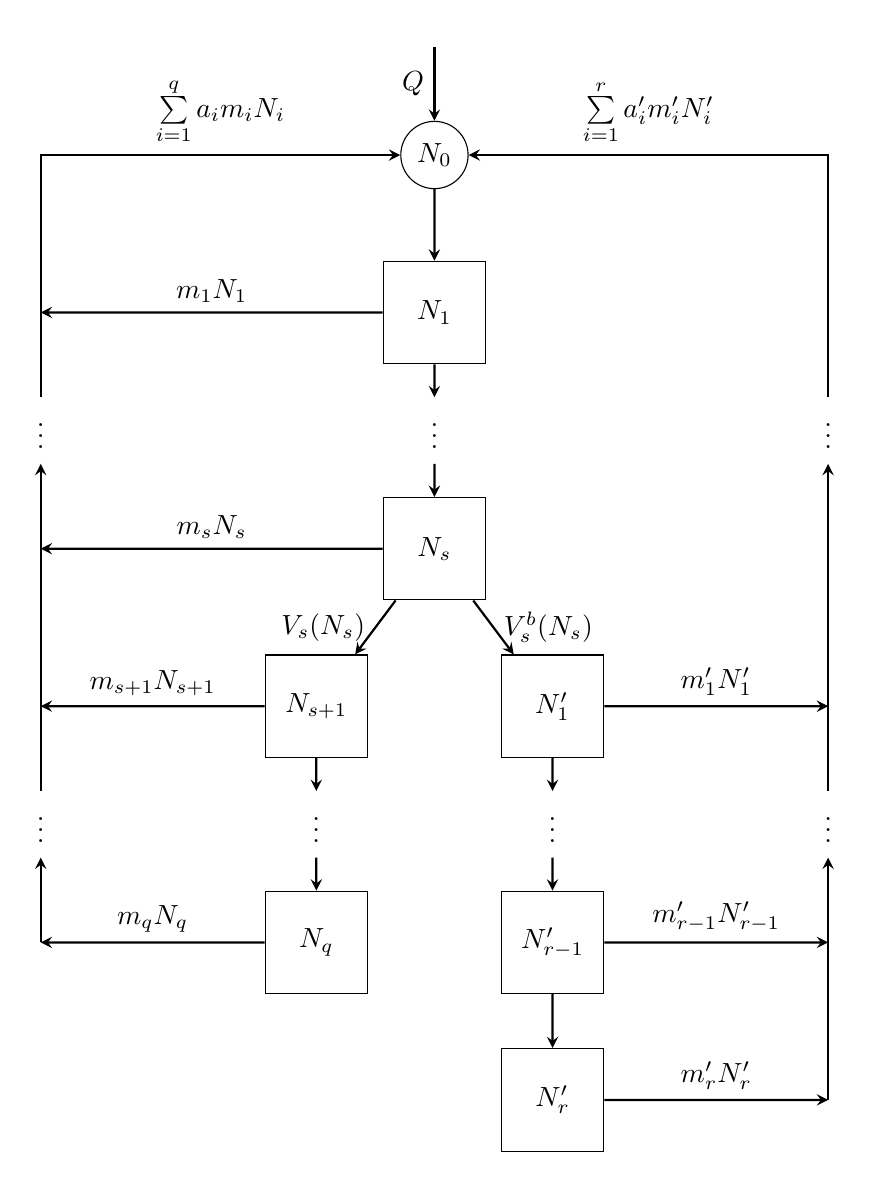
\begin{tikzpicture}

        \usetikzlibrary{shapes.geometric, calc}

        \tikzstyle{roundnode} = [draw, circle, text centered];
        \tikzstyle{squarenode} = [draw, regular polygon, regular polygon sides=4, text centered, inner sep=0, text width=0.92cm];
        \tikzstyle{arrow} = [thick, ->, >=stealth];
        

        \node[roundnode] (N0) at (0,0) {$N_0$};

        \node[squarenode] (N1) at ([yshift=-2cm]N0) {$N_1$};
        \node (ND) at ([yshift=-1.5cm]N1) {$\vdots\vphantom{lp}$};
        \node[squarenode] (NS) at ([yshift=-1.5cm]ND) {$N_s$};


        \node[squarenode] (NS1) at ([xshift=-1.5cm,yshift=-2cm]NS) {$N_{s+1}$};
        \node (NSD) at ([yshift=-1.5cm]NS1) {$\vdots\vphantom{lp}$};
        \node[squarenode] (NQ) at ([yshift=-1.5cm]NSD) {$N_q$};


        \node[squarenode] (M1) at ([xshift=1.5cm,yshift=-2cm]NS) {$N'_{1}$};
        \node (MD) at ([yshift=-1.5cm]M1) {$\vdots\vphantom{lp}$};
        \node[squarenode] (Mm1) at ([yshift=-1.5cm]MD) {$N'_{r-1}$};
        \node[squarenode] (MR) at ([yshift=-2cm]Mm1) {$N'_r$};


        \node (QN0) at ([yshift=1.5cm]N0) {};
        \draw [arrow] (QN0) -- node[anchor=east] {$Q$} (N0);

        
        \draw [arrow] (N0) -- (N1);
        \draw [arrow] (N1) -- (ND);
        \draw [arrow] (ND) -- (NS);
        
        \draw [arrow] (NS) -- node[anchor=east] {$V_s(N_s)$} (NS1);
        \draw [arrow] (NS1) -- (NSD);
        \draw [arrow] (NSD) -- (NQ);

        \draw [arrow] (NS) -- node[anchor=west] {$V^b_s(N_s)$} (M1);
        \draw [arrow] (M1) -- (MD);
        \draw [arrow] (MD) -- (Mm1);
        \draw [arrow] (Mm1) -- (MR);

        \node (DBS) at ([xshift=-5cm]ND) {$\vdots\vphantom{lp}$};
        \node (DBR) at ([xshift=5cm]ND) {$\vdots\vphantom{lp}$};
        \node (DBS2) at ($(DBS)!(NSD)!(DBS)$) {$\vdots\vphantom{lp}$};
        \node (DBR2) at ($(DBR)!(MD)!(DBR)$) {$\vdots\vphantom{lp}$};


        \draw[arrow] ($(DBS)!(NQ)!(DBS)$) -- (DBS2);
        \draw[arrow] (DBS2) -- (DBS);
        \draw[arrow] (DBS) |- node[pos=0.75, anchor=south] {$\textstyle\sum\limits_{i=1}^q a_i m_i N_i$} (N0);


        \draw[arrow] ($(DBR)!(MR)!(DBR)$) -- (DBR2);
        \draw[arrow] (DBR2) -- (DBR);
        \draw[arrow] (DBR) |- node[pos=0.75, anchor=south] {$\textstyle\sum\limits_{i=1}^r a'_i m'_i N'_i$} (N0);


        \draw[arrow] (N1) -- node[anchor=south] {$m_1 N_1$} ($(DBS)!(N1)!(DBS)$);
        \draw[arrow] (NS) -- node[anchor=south] {$m_s N_s$} ($(DBS)!(NS)!(DBS)$);
        \draw[arrow] (NS1) -- node[anchor=south] {$m_{s+1} N_{s+1}$} ($(DBS)!(NS1)!(DBS)$);
        \draw[arrow] (NQ) -- node[anchor=south] {$m_q N_q$} ($(DBS)!(NQ)!(DBS)$);
        

        \draw[arrow] (M1) -- node[anchor=south] {$m'_1 N'_1$} ($(DBR)!(M1)!(DBR)$);
        \draw[arrow] (Mm1) -- node[anchor=south] {$m'_{r-1} N'_{r-1}$} ($(DBR)!(Mm1)!(DBR)$);
        \draw[arrow] (MR) -- node[anchor=south] {$m'_{r} N'_{r}$} ($(DBR)!(MR)!(DBR)$);

    \end{tikzpicture}
    \caption{Схема ветвящейся трофической цепи с двумя ветвями. Виды \(N_i\) -- главная цепь, \(N'_i\) -- боковая.} \label{schema_split}
\end{figure}

По схеме можем построить систему дифференциальных уравнений.
\begin{equation} \label{double_full}
    \begin{split}
        & \frac{d N_0}{dt} = Q - V_0(N_0) N_1 + \sum_{i=1}^q a_i m_i N_i + \sum_{i=1}^r a'_i m'_i N'_i, \\
        & \frac{d N_i}{dt} = -m_i N_i + k_i V_{i-1}(N_{i-1}) N_i - V_i(N_i) N_{i+1}, \quad i=\overline{1,s-1},  \overline{s+1,q}, \\
        & \frac{d N_s}{dt} = -m_s N_s + k_s V_{s-1}(N_{s-1}) N_s - V_s(N_s) N_{s+1} - V_s^b(N_s) N'_1, \\
        & \frac{d N'_1}{dt} = -m'_1 N'_1 + k'_1 V_s^b(N_s) N'_1 - V'_1(N'_1) N'_{2}, \\
        & \frac{d N'_k}{dt} = -m'_k N'_k + k'_k V'_{k-1}(N'_{k-1}) N'_k - V'_k(N'_k) N'_{k+1}, \quad k=\overline{2,r}.
    \end{split}
\end{equation} 
Здесь аналогично \(N_{q+1} \equiv 0, N'_{r+1} \equiv 0\).

    \pagebreak

    \subsection{Качественная устойчивость}
    Для дальнейшего анализа устойчивости трофических цепей понадобится определение такого свойства сообществ, как \textit{качественная устойчивость}.

    \textit{Вольтеррвоская} модель сообществ \(n\) видов имеет систему вида
    \begin{equation}
        \frac{d N_i}{d t} = N_i \left( \varepsilon_i - \sum_{j=1}^{n} \gamma_{ij} N_j \right), \quad i=\overline{1,n},
    \end{equation}
    где \(\varepsilon_i\) -- скорость естественного прироста или смертности \(i\)-го вида в отсутствие всех остальных видов, а знак и абсолютная величина \(\gamma_{ij} (i \neq j)\) отражают соответственно характер и интенсивность влияния \(j\)-го вида на \(i\)-вид. \(\gamma_{ii}\) -- показатель внутривидового взаимодействия для \(i\)-го вида. Матрицу \(\Gamma = \Vert \gamma_{ij} \Vert\), отражающую структуру связей сообщества называют \textit{матрицей сообщества}.

    Для описания только характера связей введём \textit{знаковую матрицу} \(S\). Тогда она связана с матрицей сообщества соотношением 
    \[
        S = -\sign \Gamma = \left\Vert - \sign \gamma_{ij} \right\Vert
    \]

    \begin{definition}
        \textbf{Качественная устойчивость сообщества} -- сохранение устойчивости при любых количественных значениях элементов матрицы \(\Gamma = \Vert \gamma_{ij} \Vert\), сохраняющих лишь тип взаимодействия между каждой парой видов.
    \end{definition}

    Иными словами, качественная устойчивость означает, что сообщество остаётся устойчивым при любых интенсивностях  всех существующих в нем взаимодействий.

    Пусть динамика сообщества \(n\) видов описывается системой уравнений общего вида
    \begin{equation} \label{generic_n}
        \frac{d N_i}{d t} = f_i(N), \quad i = \overline{1,n},
    \end{equation}
    с функциями \(f_i (N_i)\) допускающими существование равновесия \(N^* > 0\) и линеаризацию в этой точке, то структура соотношений в сообществе может быть определена по матрице системы (\ref{generic_n}), линеаризованной в точке \(N^*\):
    \begin{equation}
        A = \left\Vert \left. \frac{\D f_i (N)}{\D N_j} \right|_{N^*} \right\Vert.
    \end{equation}
    Эта матрица является \textit{матрицей сообщества}. Она описывает характер и интенсивность взаимодействий между видами. Знаковая матрица \(S\) будет равна
    \begin{equation} \label{sign_partial}
        S = \sign A = \left\Vert \sign \frac{\D f_i (N)}{\D N_j} \right\Vert.
    \end{equation}

    Очевидно, что качественная устойчивость является лишь свойством знаковой структуры \(S\) матрицы сообщества \(A\) и на основании (\ref{sign_partial}) может быть сформулирована на языке матриц.
    \begin{definition}
        \textbf{Качественной устойчивостью матрицы} \(A\) (или знак- \hspace{-2pt}устойчивостью) называется устойчивость матрицы \(A\) при любых значениях абсолютных величин её ненулевых элементов.
    \end{definition}
    Иными словами, \(A\) сохраняет устойчивость при любых численных изменениях её элементов, не нарушающих знаковую структуру \(S = \sign A\).

    Если \(A\) не обладает знак-устойчивостью, то в рамках заданной структуры при некотором наборе \({a_{ij}}\) в спектре \(A\) обнаружатся \(\Rez \lambda_i \geq 0\), при этом может существовать такой набор, что матрица окажется устойчивой.

    Знаковым матрицам \(S\) можно поставить взаимно однозначное соответствие \textit{знаковый ориентированный граф} (далее для краткости ЗОГ). Этого можно добиться, если проводить ориентированные рёбра и приписывать им знаки \(+\) или \(-\) по правилу: если вид \(j\) влияет каким-либо образом на вид \(i\), то проводится ребро \(j \to i\) и ему приписывается знак этого влияния. 

    Таким образом, условия качественной устойчивости могут формулироваться как в терминах матриц, так и в терминах соответствующих ЗОГ.

    \subsubsection{Необходимые условия}

    Рассмотрим необходимые условия знак-устойчивости матрицы \(A\) \cite{quirk_rupert}:
    \begin{enumerate}
        \item \(a_{ij} a_{ji} \leq 0 \quad \forall i \neq j\); \label{sign_nes_1}
        \item для любой последовательности индексов \(i_1 \neq i_2 \neq i_e \neq \dots i_m \), \(m > 2\) неравенства \(a_{i_1 i_2} \neq 0, a_{i_2 i_3} \neq 0, \dots, a_{i_{m-1} i_m} \neq 0\) влекут \(a_{i_m i_1} = 0\); \label{sign_nes_2}
        \item \(a_{ii} \leq 0 \quad \forall i, \quad \exists i_0 : a_{i_0 i_0} < 0\); \label{sign_nes_3}
        \item существует ненулевой член в разложении \(\det A\). \label{sign_nes_4}
        \item матрица \(A\) является действительной и неразложимой; \label{sign_nes_neraz}
    \end{enumerate}
    С биологической точки зрения эти условия интерпретируются так: (\ref{sign_nes_1}) означает, что в сообществе не должно быть отношений конкуренции или симбиоза. (\ref{sign_nes_3}) означает, что не должно быть самовозрастающих видов и по крайней мере один вид обладает самодемпфированием. Условие (\ref{sign_nes_2}) означает, что ЗОГ сообщества не содержит ориентированных циклов длиной более 2.

    Условие (\ref{sign_nes_4}) формально означает, что есть такая перестановка \(\sigma\) индексов \(1,2,\dots,n\) такая, что произведение элементов \(s_{ij}\) знаковой матрицы \(S = \sign A\) ненулевое:
    \begin{equation} \label{sign_prod}
        s_{1, \sigma(1)} s_{2, \sigma(2)} \cdots s_{n, \sigma(n)} \neq 0.
    \end{equation}

    Известно, что любая перестановка может быть представлена в виде композиции непересекающихся циклов
    \begin{equation*}
        \sigma = c_1 \cdots c_p
    \end{equation*}
    с циклами \(c_j\) длины \(l_j\) такой, что 
    \begin{equation*}
        1 \leq l_j \leq n, \quad \sum_{j=1}^{p} l_j = n.
    \end{equation*}

    Каждому циклу \(c = (i_1, i_2, \dots, i_l)\) длины \(l\) соответствует группа ненулевых сомножителей произведения (\ref{sign_prod}):
    \begin{equation*}
        a_{i_1 i_2} \neq 0, \, a_{i_2 i_3} \neq 0, \, \dots, \, a_{i_{l-1} i_{l}} \neq 0, \, a_{i_l i_1} \neq 0.
    \end{equation*}
    Это соответствует тому, что в ЗОГ вершины \(i_1, \dots, i_l\) соединены в ориентированный цикл. В итоге, условие (\ref{sign_nes_4}) означает, что существует хотя бы одно разбиение ЗОГ на непересекающиеся циклы, сумма длин которых равна \(n\).

    Можно отметить, что учитывая условие (\ref{sign_nes_2}), запрещающее циклы длиннее 2, и (\ref{sign_nes_1}), в ЗОГ качественно устойчивого сообщества можно выделить \(k\) \( \left( 0 \leq k \leq \frac{n}{2} \right)\) пар видов хищник-жертва так, чтобы остальные \(n - 2k\) видов были самодемпфируемыми (являясь циклами длины 1).

    Существенным моментом является условие (\ref{sign_nes_neraz}), которое требует \textit{неразложимость} матрицы. 

    \begin{definition}
        Матрица \(A\) называется \textbf{разложимой}, если некоторой перестановкой её рядов (строк и соответствующих столбцов) она может быть приведена к виду
        \begin{equation}
            A = \left\Vert \begin{matrix}
                B & 0 \\
                C & D
            \end{matrix} \right\Vert,
        \end{equation}
        где \(B\) и \(D\) -- квадратные матрицы порядков \(p\) и \(q\) \((p+q = n)\).
    \end{definition}

    Для сообщества неразложимость означает, что в нём нельзя выделить группу \(p\) \( (1 \leq p \leq n)\) видов так, чтобы они не испытывали никакого влияния со стороны остальных \(n-p\) видов. На языке графов это означает, что невозможно выбрать \(p\) вершин так, чтобы ни одна из них не служила концом стрелок, идущих от каких-либо из остальных \(n-p\) вершин. Для матриц это условие требует, чтобы в каждой строке и каждом столбце должен быть хотя бы один ненулевой недиагональный элемент.

    Для примера существенности неразложимости возьмём граф на рис. \ref{example_sign_zog_2}, который соответствует разложимой матрице
    \begin{equation}
        \left\Vert \begin{matrix}
            -a & b & c \\
            0 & 0 & -d \\
            0 & e & 0 
        \end{matrix} \right\Vert, 
        \quad a, b, c, d, e > 0.
    \end{equation}
    Для этого ЗОГ выполняются условия (\ref{sign_nes_1})--(\ref{sign_nes_4}), но он имеет в спектре пару мнимых чисел \(\lambda_{1,2} = \pm i \sqrt{de} ~~ (\lambda_3 = -a)\), т.е. не является устойчивой.
    
    \begin{figure}[H]
        \centering
        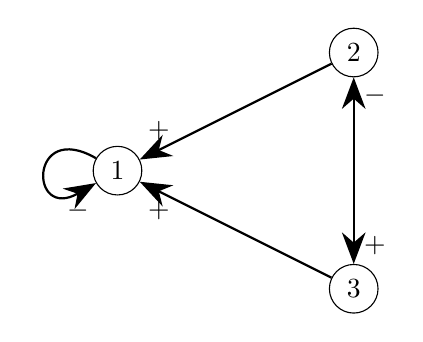
\begin{tikzpicture}
    
            \tikzstyle{roundnode} = [draw, circle, text centered];
            \tikzstyle{squarenode} = [draw, regular polygon, regular polygon sides=4, text centered, inner sep=0];
            \tikzstyle{arrow} = [thick, -{Stealth[length=4mm]}];
            \tikzstyle{arrow2} = [thick, {Stealth[length=4mm]}-{Stealth[length=4mm]} ];

            \node[roundnode] (1) at (0,1.5) {$1$};
            \node[roundnode] (2) at (3,3) {$2$};
            \node[roundnode] (3) at (3,0) {$3$};

            \draw [arrow2] (2) -- node[pos=0.1, anchor=west] {$-$} node[pos=0.9, anchor=west] {$+$} (3);
            \draw [arrow] (3) -- node[pos=0.9, anchor=north] {$+$} (1);
            \draw [arrow] (2) -- node[pos=0.9, anchor=south] {$+$} (1);

            \draw[arrow] (1) edge [out=150, in=-150, looseness=8] node [pos=0.9, anchor=north] {$-$} (1);
    
        \end{tikzpicture}
        \caption{Самолимитируемый вид-комменсал \(1\) (питается другим видом без вреда) связан с парой хищник--жертва \(3\)--\(2\).} \label{example_sign_zog_2}
    \end{figure}

    Условие неразложимости ещё более сужает разнообразие видовых соотношений. Этот факт вытекает из нижеследующей леммы. Для этого введём понятия: матрица \(A\) обладает \textit{симметричной структурой}, если \(\forall i \neq j : a_{ij} \neq 0 \Rightarrow a_{ji} \neq 0 \), и \textit{ассиметричной структурой}, если \(\exists i \neq j : a_{ij} = 0, a_{ji} \neq 0 \).

    \begin{lemma}
        Если \(A\) удовлетворяет условию (\ref{sign_nes_2}) и обладает асимметричной структурой, то \(A\) разложима. \cite{svilog}
    \end{lemma}

    Из этой леммы и условия (\ref{sign_nes_1}) следует, что симметричные ненулевые элементы неразложимой знак-устойчивой матрицы \(A\) должны иметь противоположные знаки, т.е. единственным типом межвидовых отношений в качественно устойчивом сообществе с неразложимой матрицей могут быть лишь отношения хищник--жертва. 

    Рассмотрим сообщество из 5 видов, ЗОГ которого изображён на рис. \ref{example_sign_unstable_zog}, а матрица выглядит так:
    \begin{equation}
        A = \left\Vert \begin{matrix}
            0 & 1 & 0 & 0 & 0 \\
            -1& 0 & 1 & 0 & 0 \\
            0 &-1 &-1 & 1 & 0 \\
            0 & 0 &-1 & 0 & 1 \\
            0 & 0 & 0 &-1 & 0
        \end{matrix} \right\Vert.
    \end{equation}
    
    Как легко убедиться, матрица \(A\) удовлетворяет всем условиям (\ref{sign_nes_1})--(\ref{sign_nes_4}), и, как показывает граф на рисунке \ref{example_sign_unstable_zog}, является неразложимой (\ref{sign_nes_neraz}).

    \begin{figure}[H]
        \centering
        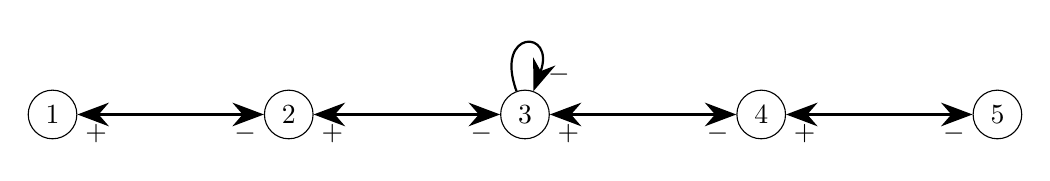
\begin{tikzpicture}
    
            \tikzstyle{roundnode} = [draw, circle, text centered];
            \tikzstyle{squarenode} = [draw, regular polygon, regular polygon sides=4, text centered, inner sep=0];
            \tikzstyle{arrow} = [thick, -{Stealth[length=4mm]}];
            \tikzstyle{arrow2} = [thick, {Stealth[length=4mm]}-{Stealth[length=4mm]} ];

            \node[roundnode] (1) at (0,0) {$1$};
            \node[roundnode] (2) at (3,0) {$2$};
            \node[roundnode] (3) at (6,0) {$3$};
            \node[roundnode] (4) at (9,0) {$4$};
            \node[roundnode] (5) at (12,0) {$5$};

            \draw [arrow2] (1) -- node[pos=0.1, anchor=north] {$+$} node[pos=0.9, anchor=north] {$-$} (2);
            \draw [arrow2] (2) -- node[pos=0.1, anchor=north] {$+$} node[pos=0.9, anchor=north] {$-$} (3);
            \draw [arrow2] (3) -- node[pos=0.1, anchor=north] {$+$} node[pos=0.9, anchor=north] {$-$} (4);
            \draw [arrow2] (4) -- node[pos=0.1, anchor=north] {$+$} node[pos=0.9, anchor=north] {$-$} (5);
            
            \draw[arrow] (3) edge [in=70, out=110, looseness=10] node [pos=0.9, anchor=west] {$-$} (3);
    
        \end{tikzpicture}
        \caption{ЗОГ сообщества 5 видов: \(i\)-й питается \((i+1)\)-м \((i=\overline{1,4})\), при этом \(3\) вид самолимитируется.} \label{example_sign_unstable_zog}
    \end{figure}

    Однако, спектр \(A\) состоит из чисел \(\lambda_1 \approx -0.36\), \(\lambda_{2,3} \approx -0.32 \pm 1.63 i\), \(\lambda_{4,5} = \pm i\), т.е. содержит чисто мнимые числа. Этот пример показывает, что условия (\ref{sign_nes_1})--(\ref{sign_nes_neraz}) являются лишь необходимыми, но не достаточными условиями знак-устойчивости.


\subsubsection{Достаточные условия}
    Для получения достаточных условий можно усилить условие (\ref{sign_nes_3}), описывающее самолимитирующие виды.

    Для этого определим понятие <<\textit{хищного сообщества}>>. В ЗОГ заданного сообщества рассмотрим какую-нибудь вершину, включенную в цикл длины $2$ ($2$-цикл), одна из стрелок которого имеет знак \(+\), а другая \(-\). Объединим все вершины, которые связаны с данной вершиной такими \(2\)-циклами. Для новых вершин повторяем процедуру объединения с вершинами, связанными с ними теми же \(2\)-циклами. Иными словами, объединим в одно множество все виды, образующие некоторую структуру связей хищник -- жертва. Максимальное множество таких видов будем называть \textbf{хищным сообществом}, содержащим первый вид. Если какой-то вид не связан соотношением \(+ \, -\) ни с какими другими видами, то будем называть его \textit{тривиальным} хищным сообществом.

    ЗОГ на рис. \ref{example_sign_unstable_zog} содержит лишь одно хищное сообщество, включающее все виды. ЗОГ на рис. \ref{example_sign_zog_2} содержит два сообщества: тривиальное \(\{1\}\) и нетривиальное \(\{2,3\}\).

    Разбиению ЗОГ с матрицей \(A = \Vert a_{ij} \Vert\) на хищные сообщества можно поставить в соответствие матрицу \(\widetilde{A} = \Vert \widetilde{a}_{ij} \Vert\) по следующему правилу: \(\widetilde{a}_{ij} = a_{ij}\), если ребро \(a_{ij}\) принадлежит некоторому циклу, и \(\widetilde{a}_{ij} = 0\) иначе. Для ЗОГ и матриц, удовлетворяющих условиям (\ref{sign_nes_1}) и (\ref{sign_nes_2}), это означает стирание всех стрелок, связывающих хищные сообщества, а матрица \(A\) приобретает блочно-диагональный вид с блоками, соответствующими отдельным хищным сообществам. Например, для ЗОГ на рис. \ref{example_sign_zog_2} это означает стирание рёбер \(2 \to 1\) и \(3 \to 1\), а матрица \(\widetilde{A}\) принимает вид
    \begin{equation*}
        \widetilde{A} = \left\Vert \begin{array}{c|cc}
            -a & 0 & 0 \\ \hline
            0 & 0 & -d \\
            0 & e & 0 
        \end{array} \right\Vert.
    \end{equation*}

    \begin{lemma}
        Все собственные числа \(A\) и \(\widetilde{A}\) совпадают.
    \end{lemma}

    \begin{proof}
        Пусть элементу \(a_{rs} \neq 0\) соответствует стрелка графа, не принадлежащая никакому циклу (длины больше 1). Это эквивалентно тому, что любое произведение вида
        \begin{equation*}
            a_{rs} a_{sr}, \quad a_{ir} a_{rs} a_{si}, \quad a_{ij} a_{jr} a_{rs} a_{si}, \quad \dots,
        \end{equation*}
        где \(r,s,i,j,dots\) -- различные индексы, обращается в 0 (следует из (\ref{sign_nes_2})).
        Рассмотрим характеристическую матрицу \(\left\Vert A - \lambda I \right\Vert = \left\Vert a_{ij} - \delta_{ij} \lambda \right\Vert\). При её разложении, все члены, содержащие сомножитель \((a_{rs} - \delta_{rs} \lambda)\), исчезнут. То есть, если положить \(a_{rs} = 0\), то значение определителя не изменится. Таким образом,
        \begin{equation}
            \det \left\Vert A - \lambda I \right\Vert = \det \left\Vert \widetilde{A} - \lambda I \right\Vert.
        \end{equation}
    \end{proof}

    Значит по устойчивости хищного сообщества можно судить по устойчивости исходного графа. Очевидно, что для устойчивости должно соблюдаться требование 
    \begin{equation*}
        0 \neq \det A = \det \widetilde{A},
    \end{equation*}
    означающее, что все тривиальные хищные сообщества должны обладать самолимитированием.
    
    \begin{theorem}
        Если \(A\) удовлетворяет условиям (\ref{sign_nes_1})--(\ref{sign_nes_4}), то \(\Rez \lambda(\widetilde{A}) \leq 0 \), причём кратность значений с нулевой вещественной частью не превосходит \(1\).
    \end{theorem}
    \begin{proof}
        Рассмотрим отдельное хищное сообщество, включающее \(m\) видов, и соответствующую \((m \times m)\)-матрицу \(\widetilde{A}\). Воспользуемся методом Ляпунова для определения устойчивости линейной системы дифференциальных уравнений 
        \begin{equation} \label{sign_hunter_ode}
            \frac{d \mathrm{x}}{dt} = \widetilde{A} \mathrm{x}.
        \end{equation}

        Нужно построить функцию Ляпунова и определить знак её производной по \(t\). Для этого определим \(m\) \textit{положительных чисел} \(\alpha_i\) следующим образом. Положим \(\alpha_1 = 1\). Для каждого \(j\)-го вида, связанного в \(\widetilde{A}\) с \(i\)-м определим соотношение
        \begin{equation} \label{sign_conntcnted_ij}
            \alpha_j a_{ji} = -\alpha_i a_{ij}, \quad i \neq j,
        \end{equation}
        тогда для видов, связанных с \(1\)-м, имеем
        \begin{equation} \label{sign_conntcnted_to_1}
            \alpha_i = - \frac{a_{1i}}{a_{i1}} > 0
        \end{equation}
        по условию (\ref{sign_nes_1}) и построению хищного сообщества. Поскольку в графе нет замкнутых петель длины больше 2, получим все числа \(\alpha_1, \dots, \alpha_m\).

        Определим функцию
        \begin{equation} \label{sign_lyapunov_func}
            V(x_1, \dots, x_m) = \sum_{i=1}^{m} \alpha_i x_i^2,
        \end{equation}
        где действительный \(m\)-вектор \(\mathrm{x}\) является решением системы (\ref{sign_hunter_ode}). Очевидно, что данная квадратичная форма положительна определена. Найдём её производную на траекториях системы:
        \begin{equation}
            \frac{dV}{dt} = \frac{\D V}{\D \mathrm{x}} \frac{d \mathrm{x}}{dt} = \nabla V \cdot \widetilde{A} \mathrm{x} = \left( 2 \alpha_i x_i \right) \cdot \left( \sum_{j=1}^{m} a_{ij} x_j \right) = 2 \sum_{i=1}^{m} \left( \alpha_i x_i  \sum_{j=1}^{m} a_{ij} x_j \right).
        \end{equation}
        Для каждого слагаемого вида \(\alpha_i a_{ij} x_i x_j\) имеем симметричное \(\alpha_j a_{ji} x_j x_i\) и в силу соотношения (\ref{sign_conntcnted_ij}) они являются противоположными и исчезнут, оставляя только диагональные элементы. Поэтому получаем
        \begin{equation}
            \frac{dV}{dt} = 2 \sum_{i=1}^{m} \alpha_i a_{ii} x_i^2 \leq 0,
        \end{equation}
        поскольку \(a_{ii} \leq 0\).

        Функция \(V\) является функцией Ляпунова для нулевого решения системы (\ref{sign_hunter_ode}) поскольку она:
        \begin{enumerate}
            \item непрерывная вместе с частными производными на \(\mathbb{R}^m\).
            \item \(V(0, \dots, 0) = 0\);
            \item \( V(x) > 0, x\neq 0 \).
        \end{enumerate}
        Следовательно, нулевое решение локально устойчиво. Поэтому \(\Rez \lambda(\widetilde{A}) \leq 0\).
        
    \end{proof}

    \pagebreak

    \section{Незамкнутая трофическая цепь}
    \subsection{Незамкнутая трофическая цепь}
    \subsubsection{Равновесные состояния}
        Поскольку единственное положительное слагаемое, которое описывает вносимое количество биомассы, в каждой строке зависит от количества биомассы предыдущего вида, то можно сделать вывод, что если в каком-то состоянии равновесия будет вид с нулевой биомассой, то и все последующие виды так же окажутся вымершими.

        Поэтому в системе (\ref{flow}) при \(Q > 0\) могут существовать \( n \) равновесных состояний типа \(\left[ N_0, N_1, \ldots, N_q, 0, \ldots, 0 \right]\), которые можно определить из уравнений
        \begin{equation} \label{flow_stationary_equations}
            \frac{dN}{dt} = 0 \Rightarrow
            \left\lbrace\begin{split}
                & N_1 = \frac{Q}{\alpha_0 N_0}, \\
                & \alpha_i N_{i+1} = k_i \alpha_{i-1} N_{i-1} - m_i, \quad i=\overline{1,q}                
            \end{split}\right.
        \end{equation}

        Из условия \( N_{q+1} = 0 \) вытекает, что 
        \begin{equation}
            N_{q-1} = \frac{m_q}{\alpha_{q-1} k_q}.
        \end{equation}

        Отметим, что в уравнениях (\ref{flow_stationary_equations}) есть связь только между \((i+1)\) и \((i-1)\) уравнениями (кроме \(0\) и \(1\)), поэтому формулы вычисления будут зависеть от чётности \(q\).

        Введём обозначения:
        \begin{equation} \label{flow_sub}
            \begin{split}
            & g_i = \frac{k_i \alpha_{i-1}}{\alpha_i}, \quad \mu_i = \frac{m_i}{\alpha_i}, \quad
            H_{2s-1} = g_1 g_3 \cdots g_{2s-1}, \quad H_{2s} = g_2 g_4 \cdots g_{2s}, \\
            & f_{2s-1} = \frac{\mu_1}{H_1} + \frac{\mu_3}{H_3} + \cdots + \frac{\mu_{2s-1}}{H_{2s-1}}, \quad
            f_{2s} = \frac{\mu_2}{H_2} + \frac{\mu_4}{H_4} + \cdots + \frac{\mu_{2s}}{H_{2s}}.
            \end{split}
        \end{equation}

        Последовательно выражая значения \(N_{i}\) имеем
        \begin{equation*}
            \begin{split}
                & N_{i} = \frac{k_{i-1} \alpha_{i-2}}{\alpha_{i-1}} N_{i-2} - \frac{m_{i-1}}{\alpha_{i-1}} = g_{i-1} N_{i-2} - \mu_{i-1} =\\ 
                &= g_{i-1} \left( g_{i-3} N_{i-4} - \mu_{i-3} \right) - \mu_{i-1} = g_{i-1} g_{i-3} N_{i-4} - g_{i-1} \mu_{i-3} - \mu_{i-1} = \dots ;
            \end{split}
        \end{equation*}

        Пусть \(i = 2s\), тогда
        \begin{equation} \label{flow_2s}
            \begin{split}
            & N_{2s} = ( g_{2s-1} g_{2s-3} \cdots g_1 ) N_0 - ( g_{2s-1} \cdots g_3 ) \mu_1 - ( g_{2s-1} \cdots g_5 ) \mu_3 - \cdots - \\
            & - g_{2s-1} \mu_{2s-3} - \mu_{2s-1} = g_{2s-1} \cdots g_1 \left( N_0 - \frac{\mu_1}{g_1} - \dots - \frac{\mu_{2s-1}}{g_1 \cdots g_{2s-1}} \right) = \\
            & = H_{2s-1} \left( N_0 - \frac{\mu_1}{H_1} - \dots - \frac{\mu_{2s-1}}{H_{2s-1}} \right)
            = H_{2s-1} \left( N_0 - f_{2s-1} \right).
            \end{split}
        \end{equation}
        Аналогично получаются значения при \(i = 2s + 1\): 
        \begin{equation} \label{flow_2s1}
            N_{2s+1} = H_{2s} (N_1 - f_{2s}).
        \end{equation}
        Здесь \( s=1,2,\ldots \)

        Для вычисления всех значений не хватает формулы для \(N_0\) или \(N_1\). Отдельно рассмотрим два случая чётности.
        \begin{enumerate}
            \item Пусть \(q = 2s\) -- \textit{чётное}. Тогда
            \begin{equation*}
                N_{q-1} = N_{2s-1} = \frac{m_{2s}}{\alpha_{2s-1} k_{2s}} \frac{\alpha_{2s}}{\alpha_{2s}} = \frac{\mu_{2s}}{g_{2s}}, \quad N_{2s-1} = H_{2s-2} (N_1 - f_{2s-2}).
            \end{equation*}
            Откуда получаем
            \begin{equation*}
                N_1 = \frac{\mu_{2s}}{g_{2s} H_{2s-2}} + f_{2s-2} = \frac{\mu_{2s}}{H_{2s}} + f_{2s-2} = f_{2s}.
            \end{equation*}
            Используя первое уравнение в (\ref{flow_stationary_equations}), будем иметь
            \begin{equation*}
                N_0 = \frac{Q}{\alpha_0 N_1} = \frac{Q}{\alpha_0 f_{2s}}.
            \end{equation*}

            \item Пусть \(q = 2s+1\) -- \textit{нечётное}. Аналогично предыдущему получаем
            \begin{equation*}
                N_{q-1} = N_{2s} = \frac{m_{2s+1}}{\alpha_{2s} k_{2s+1}} \frac{\alpha_{2s+1}}{\alpha_{2s+1}} = \frac{\mu_{2s+1}}{g_{2s+1}}, \quad N_{2s} = H_{2s-1} (N_0 - f_{2s-1}).
            \end{equation*} 
            откуда
            \begin{equation*}
                N_0 = \frac{\mu_{2s+1}}{g_{2s+1} H_{2s-1}} + f_{2s-1} = f_{2s+1}, \quad N_1 = \frac{Q}{\alpha_0 f_{2s+1}}.
            \end{equation*}
        \end{enumerate}

        Теперь легко можно получить явные выражения \(N_i\), подставив \(N_0\) и \( N_1\) в (\ref{flow_2s}) и (\ref{flow_2s1}).

        Очевидно, что стационарные значения численностей \(N_i\) имеют смысл, только когда они положительные.

        \begin{statement}
            Если в \textbf{незамкнутой} трофической цепи длины \(q\) численность \(N_q > 0\), то \(N_i > 0 \, (i=\overline{1,q-1})\).
        \end{statement}

        \begin{proof}
            Для начала заметим, что \(f_{2s}\) и \(f_{2s+1}\) положительны и монотонно возрастают с увеличением \(s\). Величины \(N_0\) и \(N_1\) также положительны и зависят от параметра \(q\) -- длины трофической цепи.  
            Поскольку все параметры положительные, то численность \( N_{q-1} > 0 \).

            Из условия \( N_q > 0 \) и (\ref{flow_2s}, \ref{flow_2s1}) получим неравенство
            \begin{equation} \label{flow_lower}
                Q > \alpha_0 f_{q-1} f_{q}
            \end{equation} 

            Предположим противное: \(\exists p < q : N_p \leq 0\). Возможны 4 варианта: \(p\) и \(q\) одинаковой чётности и разной чётности.

            \begin{enumerate}
                \item Пусть \(q = 2s \) и \( N_0 = \frac{Q}{\alpha_0 f_{2s}}, N_1 = f_{2s}\).
                \begin{enumerate}
                    \item \(p = 2u \, (u < s)\), тогда из (\ref{flow_2s}) следует, что \( N_p = N_{2u} \leq 0 \), если \(N_0 \leq f_{2u-1}\). Значит \(Q \leq \alpha_0 f_{2u-1} f_{2s} \). Сравнивая с (\ref{flow_lower}) получаем
                    \begin{equation*}
                        \alpha_0 f_{2s-1} f_{2s} < Q \leq \alpha_0 f_{2u-1} f_{2s} \Rightarrow f_{2s-1} < f_{2u-1}.
                    \end{equation*}
                    Это невозможно, поскольку \(f_{2s-1}\) монотонно возрастает с ростом \(s\).

                    \item \(p = 2u+1 \, (2u < 2s-1)\), тогда из (\ref{flow_2s1}) следует, что \( N_p = N_{2u+1} \leq 0 \) при \(N_1 \leq f_{2u}\), т.е. \(f_{2s} \leq f_{2u} \). Что также невозможно из-за монотонного возрастания \(f_{2s}\) с ростом \(s\). 
                \end{enumerate}

                \item Пусть \( q = 2s+1 \) и \( N_0 = f_{2s+1}, N_1 = \frac{Q}{\alpha_0 f_{2s+1}}\).
                \begin{enumerate}
                    \item \(p = 2u \, (2u-1 < 2s)\), тогда \( N_p = N_{2u} \leq 0 \) при \(N_0 \leq f_{2u-1}\). Значит \(f_{2s+1} < f_{2u-1} \). 
                    
                    Это невозможно, поскольку \(f_{2s-1}\) монотонно возрастает с ростом \(s\).

                    \item \(p = 2u+1 \, (u < s)\), тогда \( N_p = N_{2u+1} \leq 0 \) при \(N_1 \leq f_{2u}\), т.е. \( Q \leq \alpha f_{2u} f_{2s+1} \). Сравнивая с (\ref{flow_lower}) получаем
                    \begin{equation*}
                        \alpha_0 f_{2s} f_{2s+1} < Q \leq \alpha f_{2u} f_{2s+1} \Rightarrow f_{2s} < f_{2u}.
                    \end{equation*}
                    Что также невозможно из-за монотонного возрастания \(f_{2s}\) с ростом \(s\). 
                \end{enumerate}
            \end{enumerate}
        \end{proof}
        
        \begin{corollary}
            Из (\ref{flow_lower}) следует, что если длина трофической цепи равна \(q\), то скорость поступления ресурса \( Q \) должна превосходить критическое значение 
            \begin{equation*}
                Q^* (q) = \alpha_0 f_{q-1} f_{q}.
            \end{equation*}
        \end{corollary}

        \subsubsection{Условия существования цепи фиксированной длины}

        Для определения устойчивости равновесного состояния трофической цепи длины \(q\): \(N^* = [ N_0, N_1, \dots, N_q, 0, \dots, 0 ]\) будем исследовать собственные значения матрицы системы (\ref{flow}), линеаризованной в окрестности этого состояния.
        
        Найдём матрицу якоби этой системы и подставим равновесную точку: \( \left.\frac{\partial f}{\partial N}\right|_{N^*} \) (\(f\) -- правая часть системы). Получим матрицу
        \begin{equation} \label{flow_jacobian_small}
            J = \left\Vert \begin{matrix}
                A_q & 0 \\
                0 & D_{n-q}
            \end{matrix} \right\Vert,
        \end{equation}
        где \(D_{n-q} = \diag\left\{ -m_{q+1} + k_{q+1} \alpha_q N_q, -m_{q+2}, \ldots, -m_{n} \right\}\) и \(A_q\) матрица вида:
        \begin{equation}
            A_q = \left\Vert \begin{matrix}
                   -b_0  & -d_0   &          &     0    & \\
                    b_1  & -h_1   &  -d_1    &          & \\
                         & \ddots & \ddots   &  \ddots  &          \\
                         &        & b_{q-1}  & -h_{q-1} & -d_{q-1} \\
                         &   0    &          & b_{q}    & -h_{q}  
            \end{matrix} \right\Vert
        \end{equation}
        В нашем случае 
        \begin{equation} \label{flow_jacobian_vars}
            \begin{split}
                & b_0 = \alpha_0 N_1, \quad d_0 = \alpha_0, \\
                & b_i = k_i \alpha_{i-1} N_i, \quad d_i = \alpha_i N_i, \quad h_i = 0, \quad i=\overline{1,q}.
            \end{split}
        \end{equation}
        Значение \(h_i\) следует из уравнений (\ref{flow_stationary_equations}).


        Собственные значения \(J\) равны
        \begin{equation} \label{flow_jacobian_spectrum}
            \lambda_i = \left\{ \begin{matrix}
                \lambda_i (A_q), & i=\overline{1,q}, \\
                k_{q+1} \alpha_q N_q - m_{q+1}, & i=q+1, \\
                -m_i, & i=\overline{q+2, n}. 
            \end{matrix} \right.
        \end{equation}
        Очевидно, что при \(i = \overline{q+2,n}\) выполняется условие \(\lambda = -m_i < 0\). Для \(\lambda_{q+1}\) все переменные положительные и достаточно выполнения неравенства
        \begin{equation} \label{flow_nq_upper}
            N_q < \frac{m_{q+1}}{\alpha_q k_{q+1}}.
        \end{equation}
        Это условие становится излишним, при \(q = n\), поскольку тогда устойчивость определяется собственными значениями матрицы \(A_q\).

        Для определения устойчивости матрицы \(A_q\) воспользуемся достаточными условиями знак-устойчивости. 
        
        \textcolor{red}{Нужно добавить часть со знак-устойчивостью и др. уст. из главы 4.} \dots

        Таким образом матрица \(A_q\) удовлетворяет достаточным условием знак-устойчивости и поэтому устойчива при любых значениях заданных параметров. А это значит, что равновесие \(N^*\) асимптотически устойчиво.

        Находя явное значение \(N_q\) для чётного и нечётного \(q\) и используя (\ref{flow_nq_upper}) получим:
        \begin{enumerate}
            \item При \(q = 2s\):
            \begin{equation}
                \begin{split}
                    & N_{2s} = H_{2s-1} \left( \frac{Q}{\alpha_0 f_{2s}} - f_{2s-1} \right) < \frac{m_{2s+1}}{\alpha_{2s} k_{2s+1}} \Rightarrow \\
                    & \Rightarrow \frac{Q}{\alpha_0 f_{2s}} - f_{2s-1} < \frac{m_{2s+1}}{\alpha_{2s} k_{2s+1}} \frac{\alpha_{2s+1}}{\alpha_{2s+1}} \frac{1}{H_{2s-1}} = \frac{\mu_{2s+1}}{g_{2s+1} H_{2s-1}} = \frac{\mu_{2s+1}}{H_{2s+1}} \Rightarrow \\
                    & Q < \alpha_0 f_{2s} \left(  f_{2s-1} + \frac{\mu_{2s+1}}{H_{2s+1}} \right) = \alpha_0 f_{2s} f_{2s+1},        
                \end{split}
            \end{equation}
            
            \item При \(q = 2s+1\):
            \begin{equation}
                \begin{split}
                    & N_{2s+1} = H_{2s} \left( \frac{Q}{\alpha_0 f_{2s+1}} - f_{2s+1} \right) < \frac{m_{2s+2}}{\alpha_{2s+1} k_{2s+2}} \Rightarrow \\
                    & \Rightarrow \frac{Q}{\alpha_0 f_{2s+1}} - f_{2s} < \frac{m_{2s+2}}{\alpha_{2s+1} k_{2s+2}} \frac{\alpha_{2s+2}}{\alpha_{2s+2}} \frac{1}{H_{2s}} = \frac{\mu_{2s+2}}{g_{2s+2} H_{2s}} = \frac{\mu_{2s+2}}{H_{2s+2}} \Rightarrow \\
                    & Q < \alpha_0 f_{2s+1} \left(  f_{2s} + \frac{\mu_{2s+2}}{H_{2s+2}} \right) = \alpha_0 f_{2s+1} f_{2s+2},      
                \end{split}
            \end{equation}
        \end{enumerate}
        объединяя получим
        \begin{equation}
            Q < \alpha_0 f_{q} f_{q+1} = Q^*(q+1).
        \end{equation}

        \begin{corollary}
            Необходимым и достаточным условием существования устойчивой незамкнутой трофической цепи длины \(q\) является ограничение (сверху и снизу) скорости поступления внешнего ресурса в экосистему:
            \begin{equation}
                Q^*(q) < Q < Q^*(q+1).
            \end{equation}.
        \end{corollary}
        
        \textcolor{green}{Нужно добавить картинки с численными эксп. с линейной моделью и моделью в общем случае.}

    % \begin{figure}[H]
    %     \centering
    %     % 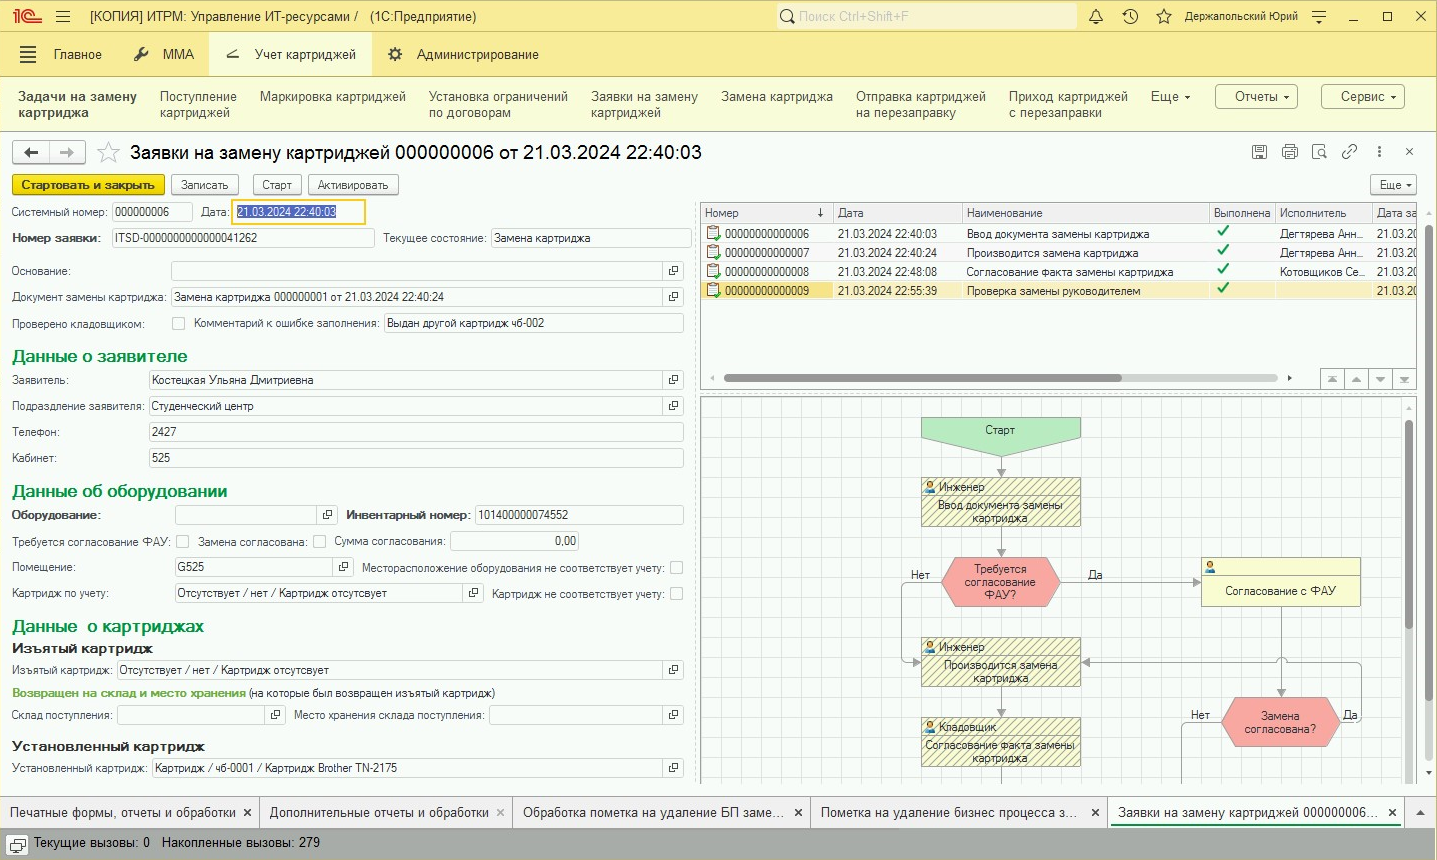
\includegraphics[width=14cm]{pictures/process.png}
    %     % \caption{}  \label{pic_label}
    % \end{figure}



    \pagebreak

    \subsection{Численные эксперименты}
Рассмотрим систему (\ref{flow}) при \(n=3\) со следующими коэффициентами:
\begin{equation} \label{flow_exp1}
    \begin{split}
        & \alpha_0 = 20, ~~ \alpha_1 = 16, ~~ \alpha_2 = 12, ~~ \alpha_3 = 8; \\
        & k_1 = 0.3, ~~ k_2 = 0.2, ~~ k_3 = 0.1; \\
        & m_1 = 4, ~~ m_2 = 3, ~~ m_3 = 2. \\ 
    \end{split}
\end{equation}
Имеем трофические цепи длиной от \(q=1\) до \(q=3\). При заданных значениях параметров имеем данные интервалы, ограничивающие поступление внешнего ресурса \(Q\):
\begin{enumerate}
    \item \(0 < Q < 12.5\);
    \item \(12.5 < Q < 95.83\ldots\);
    \item \( 95.83\ldots < Q\).
\end{enumerate}
Варьируем значение \(Q\) и получаем графики численностей в равновесии.

Для численного решения используем метод Рунге-Кутты \(4\)-порядка с шагом \(h = 0.01\). Начальные значения численностей равно \(2\).

Обозначения: <<Равн\(\{i\}\)>> -- значение точки равновесия, которой соответствует <<Вид\(\{i\}\)>>.

\begin{figure}[H]
    \centering
    \begin{subfigure}[t]{.45\linewidth}
        \centering
        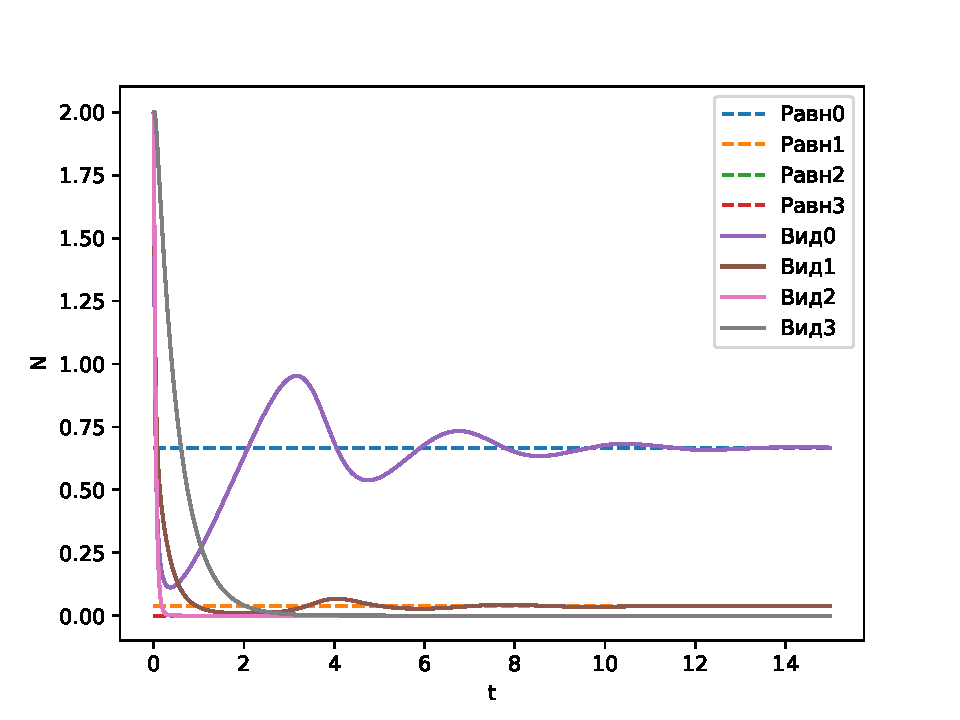
\includegraphics[width=\textwidth]{pictures/exp_flow/exp1_Q0.5.pdf}
        \caption{\(Q = 0.5\)}
    \end{subfigure}
    \begin{subfigure}[t]{.45\linewidth}
            \centering
            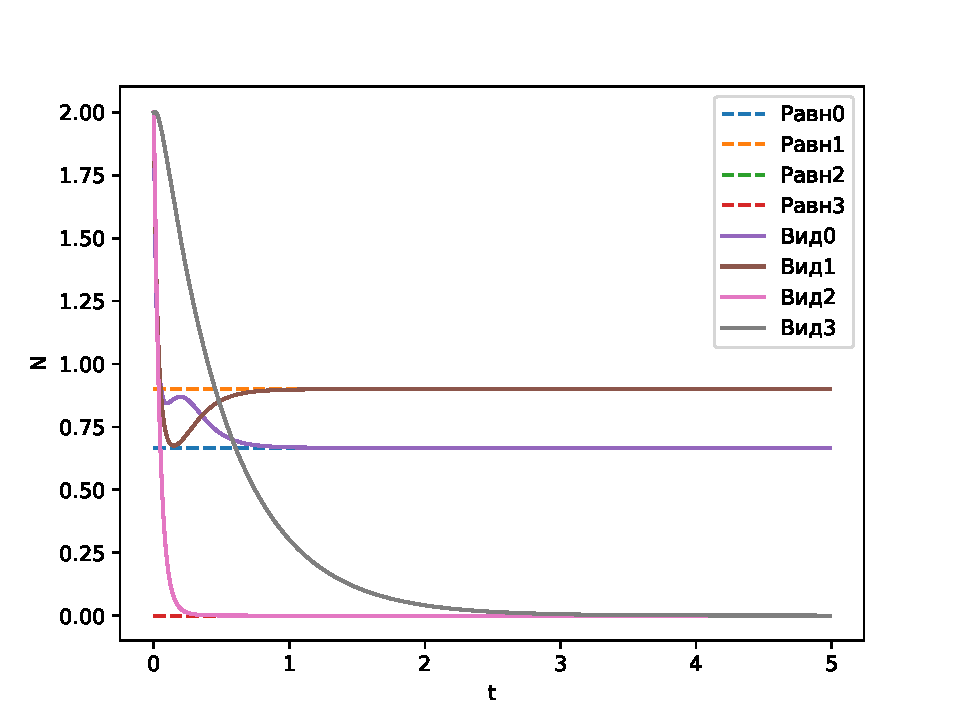
\includegraphics[width=\textwidth]{pictures/exp_flow/exp1_Q12.pdf}
            \caption{\(Q = 12\)}
        \end{subfigure}
    \caption{Численности видов системы, при \(Q\) близко к концам первого интервала.}  \label{fig:flow_exp1_q1}
\end{figure}


\begin{figure}[H]
    \centering
    \begin{subfigure}[t]{.45\linewidth}
        \centering
        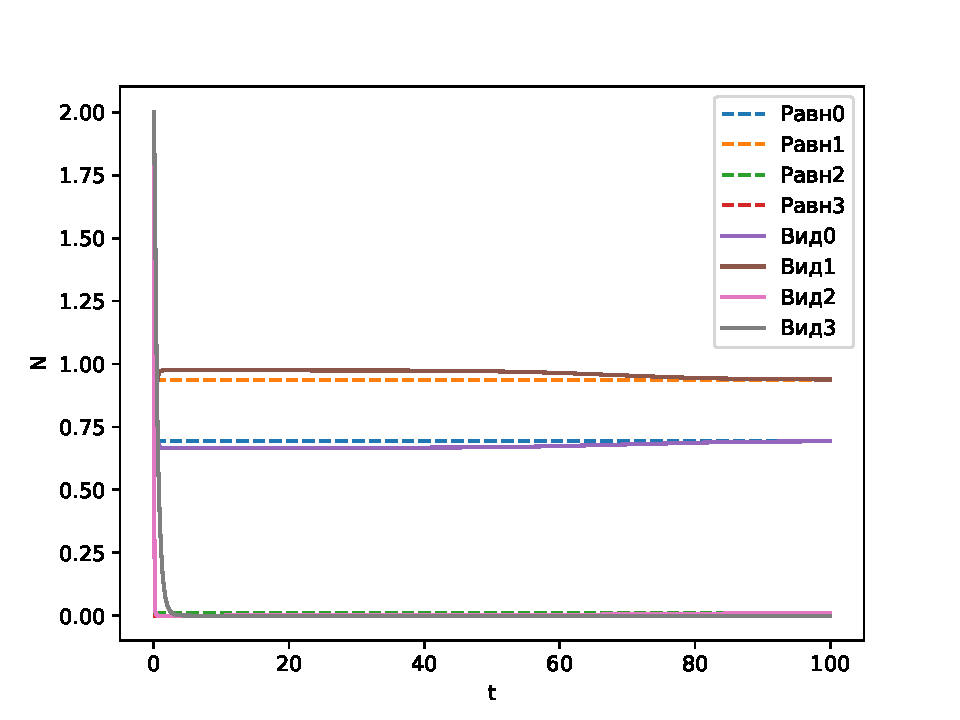
\includegraphics[width=\textwidth]{pictures/exp_flow/exp1_Q13.pdf}
        \caption{\(Q = 13\)}
    \end{subfigure}
    \begin{subfigure}[t]{.45\linewidth}
            \centering
            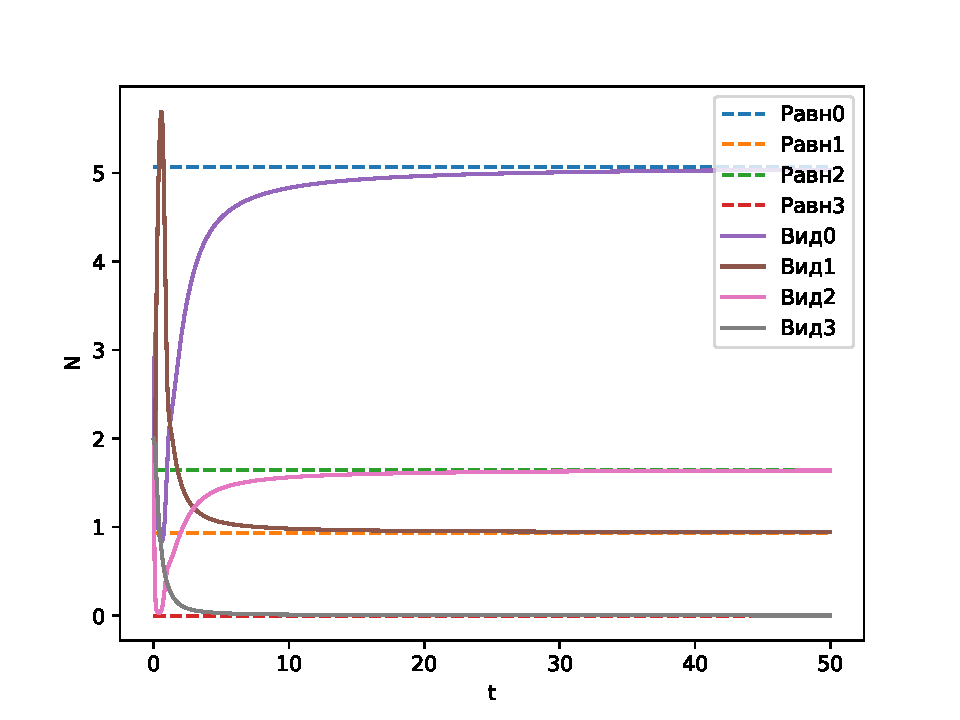
\includegraphics[width=\textwidth]{pictures/exp_flow/exp1_Q95.pdf}
            \caption{\(Q = 95\)}
        \end{subfigure}
    \caption{Численности видов системы, при \(Q\) близко к концам второго интервала.}  \label{fig:flow_exp1_q2}
\end{figure}


\begin{figure}[H]
    \centering
    \begin{subfigure}[t]{.45\linewidth}
        \centering
        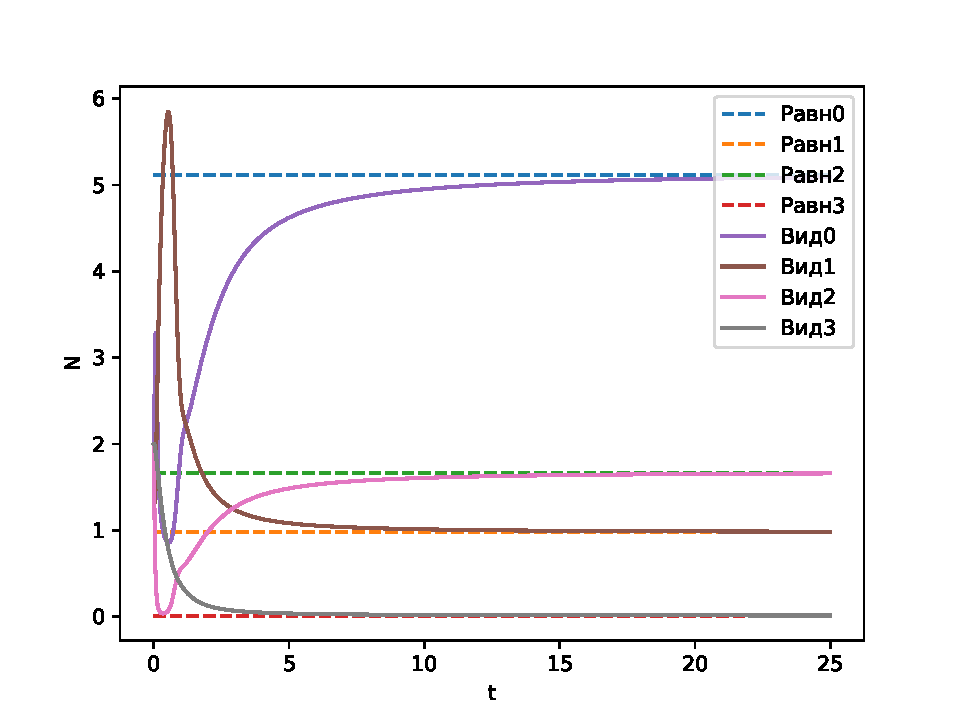
\includegraphics[width=\textwidth]{pictures/exp_flow/exp1_Q100.pdf}
        \caption{\(Q = 100, \quad N_3 \approx 0.0108\ldots \)}
    \end{subfigure}
    \begin{subfigure}[t]{.45\linewidth}
            \centering
            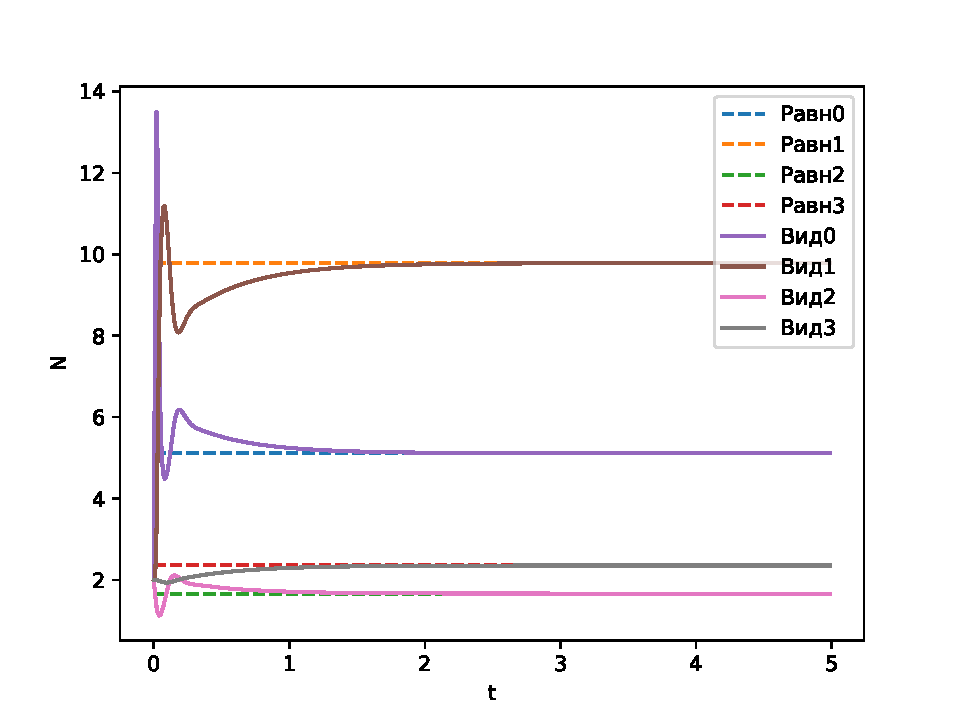
\includegraphics[width=\textwidth]{pictures/exp_flow/exp1_Q1000.pdf}
            \caption{\(Q = 1000\)}
        \end{subfigure}
    \caption{Численности видов системы, при \(Q\) близко к началу третьего интервала и на некотором отдалении.}  \label{fig:flow_exp1_q3}
\end{figure}

Как видно по графикам, модель ведёт себя в соответствии с теоретическим анализом. На каждом из интервалов ровно нужное количество видов остаётся в живых. 

Для сравнения поведения системы при <<напряжённых>> трофических связях, возьмём систему (\ref{flow_full}) при трофических функциях \( V_i(x) = \alpha_i \arctan x \). Т.е. виды могут насыщаться и не все его жертвы будут становиться добычей.


\begin{figure}[H]
    \centering
    \subfigexp{0.5}{pictures/exp_flow/exp2_Q}{.3}
    \subfigexp{17}{pictures/exp_flow/exp2_Q}{.3}
    \subfigexp{20}{pictures/exp_flow/exp2_Q}{.3}
    \subfigexp{34}{pictures/exp_flow/exp2_Q}{.3}
    \subfigexp{35}{pictures/exp_flow/exp2_Q}{.3}
    \subfigexp{40}{pictures/exp_flow/exp2_Q}{.3}
    \subfigexp{100}{pictures/exp_flow/exp2_Q}{.3}
    \subfigexp{1000}{pictures/exp_flow/exp2_Q}{.3}
\caption{Численности видов системы.}  \label{fig:flow_exp2}
\end{figure}

Как видно, с некоторого значения \(Q\) асимптотическая устойчивость прекращается и появляется периодическое поведение поведение.

    \pagebreak

    \section{Замкнутая трофическая цепь}
    \subsection{Равновесные состояния}
Аналогично незамкнутой системе, в системе с частичным восстановлением ресурса (\ref{cycle}) при \(Q > 0\) могут существовать \( n \) равновесных состояний типа \(\left[ N_0, N_1, \ldots, N_q, 0, \ldots, 0 \right]\), которые могут быть найдены из уравнений
\begin{equation} \label{cycle_stationary_equations}
    \frac{d \mb{N} }{dt} = 0 \Rightarrow
    \left\lbrace\begin{split}
        & Q + \sum_{i=1}^{q} a_i m_i N_i = \alpha_0 N_0 N_1, \\
        & \alpha_i N_{i+1} = k_i \alpha_{i-1} N_{i-1} - m_i, \quad i=\overline{1,q}                
    \end{split}\right.
\end{equation}

Поскольку связь \(N_{i-1}\) и \(N_{i+1}\) точно такая же, что и у незамкнутой модели, то значения \(N_i\) также могут быть определены по формулам (\ref{flow_2s}, \ref{flow_2s1}). Остаётся найти явные выражения для \(N_0\) и \( N_1\).

Используем обозначения (\ref{flow_sub}) и введём новые:
\begin{equation} \label{cycle_sub}
    \begin{split}
    & \varphi_s = \sum_{j=1}^{s} a_{2j} m_{2j} H_{2j-1}, \quad 
    \psi_s = \sum_{j=1}^{s} a_{2j-1} m_{2j-1} H_{2j-2}, \\
    & \sigma_i = \sum_{j=1}^{i} a_j m_j f_{j-1} H_{j-1} \quad (H_0 = 1, \, f_0 = 0).
    \end{split}
\end{equation}

\begin{enumerate}
    \item Пусть \(q = 2s\) -- \textit{чётное}. Тогда аналогично шагам для незамкнутой цепи получаем \( N_1 = f_{2s} \).
    Используя первое уравнение в (\ref{cycle_stationary_equations}), будем иметь            
    \begin{equation*}
    \begin{split}
        Q & + \sum\limits_{i=1}^{s} a_{2i-1} m_{2i-1} H_{2i-2}(N_1 - f_{2i-2}) +\\
        & + \sum\limits_{i=1}^{s} a_{2i} m_{2i} H_{2i-1}(N_0-f_{2i-1}) = \alpha_0 N_0 N_1, \\
        % Q &+ \sum\limits_{i=1}^{s} a_{2i-1} m_{2i-1} H_{2i-2}(f_{2s} - f_{2i-2}) =\\ 
        % & = \alpha_0 N_0 N_1 - \sum\limits_{i=1}^{s} a_{2i} m_{2i} H_{2i-1}(N_0-f_{2i-1}), \\
        Q &+ f_{2s} \sum\limits_{i=1}^{s} a_{2i-1} m_{2i-1} H_{2i-2} - \sum\limits_{i=1}^{s} a_{2i-1} m_{2i-1} H_{2i-2} f_{2i-2} = \\
        & = N_0 \left( \alpha_0 f_{2s} - \sum\limits_{i=1}^{s} a_{2i} m_{2i} H_{2i-1} \right) + \sum\limits_{i=1}^{s} a_{2i} m_{2i} H_{2i-1} f_{2i-1},  \\
        Q &+ f_{2s} \psi_s - \sigma_{2s} = N_0 \left( \alpha_0 f_{2s} - \varphi_s \right), \\
        N_0 &= \frac{Q + f_{2s} \psi_s - \sigma_{2s}}{\alpha_0 f_{2s} - \varphi_s}.
    \end{split}
    \end{equation*}

    \item Пусть \(q = 2s+1\) -- \textit{нечётное}. Тогда \( N_1 = f_{2s+1} \) и
    \begin{equation*}
        \begin{split}
            Q &+ \sum\limits_{i=1}^{s+1} a_{2i-1} m_{2i-1} H_{2i-2}(N_1 - f_{2i-2}) +\\
            & + \sum\limits_{i=1}^{s} a_{2i} m_{2i} H_{2i-1}(N_0-f_{2i-1}) = \alpha_0 N_0 N_1, \\
            % & Q + \sum\limits_{i=1}^{s} a_{2i} m_{2i} H_{2i-1}(f_{2s+1} - f_{2i-1}) =\\
            % &= \alpha_0 N_0 N_1 - \sum\limits_{i=1}^{s+1} a_{2i-1} m_{2i-1} H_{2i-2}(N_1 - f_{2i-2}), \\
            Q &+ f_{2s+1} \sum\limits_{i=1}^{s} a_{2i} m_{2i} H_{2i-1} - \sum\limits_{i=1}^{s} a_{2i} m_{2i} H_{2i-1} f_{2i-1} = \\
            & = N_1 \left( \alpha_0 f_{2s+1} - \sum\limits_{i=1}^{s+1} a_{2i-1} m_{2i-1} H_{2i-2} \right) + \sum\limits_{i=1}^{s+1} a_{2i-1} m_{2i-1} H_{2i-2} f_{2i-2},  \\
            Q &+ f_{2s+1} \varphi_s - \sigma_{2s+1} = N_1 \left( \alpha_0 f_{2s+1} - \psi_{s+1} \right), \\
            N_1 &= \frac{Q + f_{2s+1} \varphi_s - \sigma_{2s+1}}{ \alpha_0 f_{2s+1} - \psi_{s+1} }.
        \end{split}
        \end{equation*}
\end{enumerate}

В итоге имеем:
\begin{enumerate}
    \item \(q = 2s\): \begin{equation} \label{cycle_2s_01}
        N_1 = f_{2s}, \quad 
        N_0 = \frac{Q + f_{2s} \psi_s - \sigma_{2s}}{\alpha_0 f_{2s} - \varphi_s}
    \end{equation}
    \item \(q = 2s+1\): \begin{equation} \label{cycle_2s1_01}
        N_0 = f_{2s+1}, \quad 
        N_1 = \frac{Q + f_{2s+1} \varphi_s - \sigma_{2s+1}}{ \alpha_0 f_{2s+1} - \psi_{s+1} }
    \end{equation}
\end{enumerate}

\begin{statement}
    Если в \textbf{замкнутой} трофической цепи длины \(q\) численность \(N_q > 0\), то \(N_i > 0 \, (i=\overline{1,q-1})\).
\end{statement}

\begin{proof}
    Из условия \( N_q > 0 \) и (\ref{cycle_2s_01}, \ref{cycle_2s1_01}) получим неравенства, ограничивающие скорость поступления внешнего ресурса в систему.
    \begin{enumerate}
        \item \( q = 2s \) \begin{equation}  \label{cycle_lower_2s}
            \begin{split}
                & N_q = N_{2s} = H_{2s-1} (N_0 - f_{2s-1}) > 0, \quad 
                \frac{Q + f_{2s} \psi_s - \sigma_{2s}}{\alpha_0 f_{2s} - \varphi_s} > f_{2s-1}, \\
                & Q > \alpha_0 f_{2s-1} f_{2s} - ( \varphi_s f_{2s-1} + f_{2s} \psi_s - \sigma_{2s} ) = \widetilde{Q}^*(q).
            \end{split}
        \end{equation}
        
        \item \( q = 2s+1 \) \begin{equation}  \label{cycle_lower_2s1}
            \begin{split}
                & N_q = N_{2s+1} = H_{2s} (N_1 - f_{2s}) > 0, \quad 
                \frac{Q + f_{2s+1} \varphi_s - \sigma_{2s+1}}{ \alpha_0 f_{2s+1} - \psi_{s+1} } > f_{2s}, \\
                & Q > \alpha_0 f_{2s+1} f_{2s} - ( \psi_{s+1} f_{2s} + f_{2s+1} \varphi_s - \sigma_{2s+1}) = \widetilde{Q}^*(q).
            \end{split}
        \end{equation}
    \end{enumerate}


    Предположим противное: \(\exists p < q : N_p \leq 0\). Возможны 4 варианта: \(p\) и \(q\) одинаковой чётности и разной чётности.

    \begin{enumerate}
        \item Пусть \(q = 2s \) и \( N_0 = \frac{Q + f_{2s} \psi_s - \sigma_{2s}}{\alpha_0 f_{2s} - \varphi_s}, N_1 = f_{2s}\).
        \begin{enumerate}
            \item \(p = 2u \, (u < s)\), тогда из (\ref{flow_2s}) следует, что \( N_p = N_{2u} \leq 0 \), если \(N_0 \leq f_{2u-1}\). Значит 
            \begin{equation*}
                Q \leq f_{2u-1} ( \alpha_0 f_{2s} - \varphi_s ) - (f_{2s} \psi_s - \sigma_{2s}).
            \end{equation*}
            Сравнивая с (\ref{cycle_lower_2s}) получаем
            \begin{equation*}
                \begin{split}
                & \left\{ \begin{split}
                    & Q > f_{2s-1} ( \alpha_0 f_{2s} - \varphi_s ) - f_{2s} \psi_s + \sigma_{2s}, \\
                    & Q \leq f_{2u-1} ( \alpha_0 f_{2s} - \varphi_s ) - f_{2s} \psi_s + \sigma_{2s},
                \end{split} \right. \\
                & f_{2s-1} < f_{2u-1}
                \end{split}
            \end{equation*}
            Это невозможно, поскольку \(f_{2s-1}\) монотонно возрастает с ростом \(s\).

            \item \(p = 2u+1 \, (2u < 2s-1)\), тогда из (\ref{flow_2s1}) следует, что \( N_p = N_{2u+1} \leq 0 \) при \(N_1 \leq f_{2u}\), т.е. \(f_{2s} \leq f_{2u} \). Что также невозможно из-за монотонного возрастания \(f_{2s}\) с ростом \(s\). 
        \end{enumerate}

        \item Пусть \( q = 2s+1 \) и \( N_0 = f_{2s+1}, N_1 = \frac{Q + f_{2s+1} \varphi_s - \sigma_{2s+1}}{ \alpha_0 f_{2s+1} - \psi_{s+1} } \).
        \begin{enumerate}
            \item \(p = 2u \, (2u-1 < 2s)\), тогда \( N_p = N_{2u} \leq 0 \) при \(N_0 \leq f_{2u-1}\). Значит \(f_{2s+1} < f_{2u-1} \). 
            
            Это невозможно, поскольку \(f_{2s-1}\) монотонно возрастает с ростом \(s\).

            \item \(p = 2u+1 \, (u < s)\), тогда \( N_p = N_{2u+1} \leq 0 \) при \(N_1 \leq f_{2u} \), т.е. 
            \begin{equation*}
                Q \leq f_{2u} ( \alpha_0 f_{2s+1} - \psi_{s+1} ) - f_{2s+1} \varphi_s + \sigma_{2s+1}
            \end{equation*}
            Сравнивая с (\ref{cycle_lower_2s1}) получаем
            \begin{equation*}
                \begin{split}
                & \left\{ \begin{split}
                    & Q > f_{2s} ( \alpha_0 f_{2s+1}  - \psi_{s+1} ) - f_{2s+1} \varphi_s + \sigma_{2s+1}, \\
                    & Q \leq f_{2u} ( \alpha_0 f_{2s+1} - \psi_{s+1} ) - f_{2s+1} \varphi_s + \sigma_{2s+1},
                \end{split} \right. \\
                & f_{2s} < f_{2u}.
                \end{split}
            \end{equation*}
            Что также невозможно. 
        \end{enumerate}
    \end{enumerate}
\end{proof}

\subsection{Условия существования цепи фиксированной длины}

Линеаризуем систему (\ref{cycle}) для определения устойчивости в окрестности состояния \(N^* = [ N_0, N_1, \dots, N_q, 0, \dots, 0 ]\) .

Получим матрицу, похожую на (\ref{flow_jacobian_small}), вида
\begin{equation} \label{cycle_stability_matrix}
    J = \pares{ \begin{matrix}
        A^1_q & C \\
        0 & D_{n-q}
    \end{matrix} },
\end{equation}
где
\begin{equation}
    A^1_q = \pares{ \begin{matrix}
            -b_0  & c_1-d_0&   c_2    &  \dots   & c_q      \\
            b_1  &  0     &  -d_1    &          &  0       \\
                    & \ddots & \ddots   &  \ddots  &          \\
                    &        & b_{q-1}  &     0    & -d_{q-1} \\
                    &   0    &          & b_{q}    &  0  
    \end{matrix} }, ~
    C = \pares{ \begin{matrix}
        c_{q+1} & c_{q+2} & \dots & c_{n} \\
                &    0    &       &
    \end{matrix} },
\end{equation}
\( c_i = a_i m_i, i = \overline{1,n} \), а остальные обозначения соответствуют (\ref{flow_jacobian_vars}).

Аналогично из (\ref{flow_jacobian_spectrum}) имеем асимптотическую устойчивость системы при
\begin{align} \label{cycle_nq_upper}
    N_q < \frac{m_{q+1}}{\alpha_q k_{q+1}}.
\end{align}
и устойчивости матрицы \( A^1_q \).

Матрица \(A^1_q\) не является якобиевой (трёхдиагональной), поэтому определять её устойчивость нужно определять методами обычной устойчивости, например с помощью характеристического многочлена.

\begin{equation*}
    P_q (\lambda) = \det (A^1_q - \lambda I) = \left| \begin{matrix}
        -b_0 -\lambda & c_1-d_0&   c_2    &  \dots   & c_q      \\
            b_1  & -\lambda &  -d_1    &          &  0       \\
                & \ddots & \ddots   &  \ddots  &          \\
                &        & b_{q-1}  & -\lambda & -d_{q-1} \\
                &   0    &          & b_{q}    & - \lambda
    \end{matrix} \right|
\end{equation*}
Раскладывая определитель сначала по нижней строке, а потом по последнему столбцу получим:
\begin{equation*}
    \begin{split}
    & P_q (\lambda) = -\lambda P_{q-1} (\lambda) - b_q \left| \begin{matrix}
        -b_0 -\lambda & c_1-d_0&   c_2    &  \dots   & c_{q-2}    & c_q \\
            b_1  & -\lambda &  -d_1    &          &  & 0 \\
                & \ddots & \ddots   &  \ddots  &   \\
                &       &   b_{q-3}  & -\lambda & -d_{q-3} &   \\
                &                &    &   b_{q-2}  &   -\lambda  &      \\
                &   0           &   &     &  b_{q-1}  & -d_{q-1}  \\
    \end{matrix} \right| = \\
    & = -\lambda P_{q-1} (\lambda) - b_q( -d_{q-1} ) P_{q-2} (\lambda) -b_q (-1)^{q} c_q \left| \begin{matrix}
            b_1  & -\lambda &  -d_1    &        & 0  \\
                & \ddots & \ddots   &  \ddots  &   \\
                &       &   b_{q-3}  & -\lambda & -d_{q-3}  \\
                &  0            &    &   b_{q-2}  &   -\lambda  \\
            &                &   &  &   b_{q-1}  \\
    \end{matrix} \right| = \\
    & = -\lambda P_{q-1} (\lambda) + b_q d_{q-1} P_{q-2} (\lambda) - (-1)^{q} c_q \prod_{i=1}^{q} b_i.
    \end{split}
\end{equation*}
Учитывая начальные значения характеристического многочлена получаем рекуррентную формулу:
\begin{equation} \label{cycle_reccur}
    \begin{split}
        & P_q (\lambda) = -\lambda P_{q-1} (\lambda) + b_q d_{q-1} P_{q-2} (\lambda) - (-1)^{q} c_q b_1 \cdots b_q, \\
        & P_0 (\lambda) = - b_0 -\lambda, \\
        & P_1 (\lambda) = \lambda^2 + b_0 \lambda + b_1 (d_0 - c_1).
    \end{split}
\end{equation}

Если характеристическое уравнение \( P_q (\lambda) = 0 \) записано в виде
\begin{equation*}
    \lambda^{q+1} + e_q(\lambda) \lambda^q + e_{q-1}(\lambda) \lambda^{q-1} + \dots + e_{1}(\lambda) \lambda + e_0(q) = 0,
\end{equation*}
тогда, используя (\ref{cycle_reccur}), можно выписать рекуррентные  соотношения для коэффициентов \(e_i (q)\):
\begin{equation} \label{cycle_reccur_coeffs}
    \begin{split}
        & e_i (q) = \left\{\begin{split}
        & b_q d_{q-1} e_0(q-2) - (-1)^q c_q b_1 \cdots b_q, && i = 0, \\
        & e_{i-1} (q-1) + b_q d_{q-1} e_i (q-2), && i = \overline{1,q}, \\
        & 1, && i = q+1, \\
        & 0, && i \geq q+2, \\
    \end{split}\right. \\
    & e_{1} (1) = b_0, \\
    & e_{0} (0) = b_0, \\
    & e_{0} (1) = b_1 (d_0 - c_1).
    \end{split}
\end{equation}

Рассмотрим 2 случая.

\begin{enumerate}
\item Пусть \(q = 1\), тогда характеристический многочлен будет выглядеть как
\begin{equation*}
    \lambda^2 + e_1 (1) \lambda + e_0(1) = \lambda^2 + b_0 \lambda + b_1(d_0 - c_1) = 0.
\end{equation*}
Откуда корни уравнения
\begin{equation*}
    \lambda = \frac{-b_0 \pm \sqrt{b_0^2 - 4b_1 (d_0 - c_1)}}{2}.
\end{equation*}
Для устойчивости необходимо \(\lambda < 0\), тогда это условие эквивалентно
\begin{equation*}
    \begin{split}
        & b_0 > \sqrt{b_0^2 - 4b_1 (d_0 - c_1)}, \\
        & 0 < 4b_1 (d_0 - c_1).
    \end{split}
\end{equation*}
Значит, матрица \(A^1_1\) устойчива, если \(c_1 < d_0\), или \(m_1 a_1 < \alpha_0 N_0\). Из \eqref{cycle_2s1_01} имеем \(N_0 = \frac{m_1}{\alpha_0 k_1}\), поэтому условие устойчивости можно записать в виде \(a_1 k_1 < 1\). При этом
\begin{equation*}
    N_1 = \frac{Q + f_{1} \varphi_0 - \sigma_{1}}{ \alpha_0 f_{1} - \psi_{1} } = \frac{Q + \left( \frac{m_1}{\alpha_1} \cdot \frac{\alpha_1}{k_1 \alpha_0} \right) \cdot 0 - 0}{\alpha_0 \cdot \left( \frac{m_1}{\alpha_1} \cdot \frac{\alpha_1}{k_1 \alpha_0} \right) - a_1 m_1} = \frac{Q k_1}{m_1(1 - a_1 k_1)}.
\end{equation*}
Тогда \(N_1 > 0\) только при \(a_1 k_1 < 1\). Неравенство \eqref{cycle_nq_upper} даёт ограничение сверху на скорость поступления ресурса.
\begin{equation*}
    \begin{split}
        & \frac{Q k_1}{m_1(1 - a_1 k_1)} < \frac{m_2}{\alpha_1 k_2}, \\
        & Q < \frac{m_1 m_2}{\alpha_1 k_1 k_2} (1 - a_1 k_1) = \wt{Q}^*(2).        
    \end{split}
\end{equation*}
Таким образом, ограничение скорости поступления ресурса
\begin{equation*}
    0 < Q < \frac{m_1 m_2}{\alpha_1 k_1 k_2} (1 - a_1 k_1)
\end{equation*}
является необходимым и достаточным условием существования устойчивого равновесия типа \([N_0, N_1, 0, \dots, 0]\), то есть существования замкнутой трофической цепи длины \(1\).

\item Пусть \(q=2\), тогда имеем \( \lambda^3 + e_2(2) \lambda^2 + e_1(2) \lambda + e_0(2) = 0 \). По теореме Виета корни связаны соотношениями:
\begin{equation*}
    \begin{split}
        & \lambda_1 + \lambda_2 + \lambda_3 = -e_2(2), \\
        & \lambda_1 \lambda_2 + \lambda_2 \lambda_3 + \lambda_1 \lambda_3 = e_1(2), \\
        & \lambda_1 \lambda_2 \lambda_3 = -e_0(2).
    \end{split}
\end{equation*}
Для устойчивости нужно \(\lambda_i < 0\), значит \( e_0(2), e_1(2), e_2(2) > 0 \). С помощью формул \eqref{cycle_reccur_coeffs} получим
\begin{equation*}
    \begin{split}
        & e_0(2) = b_2 d_{1} e_0(0) - c_2 b_1 b_2 = b_2 ( d_{1} b_0 - c_2 b_1 ) > 0, \\
        & e_1(2) = e_0(1) + b_2 d_1 e_1(0) = b_1 (d_0 - c_1) + b_2 d_1 \cdot 1 > 0, \\
        & e_2(2) = e_1(1) + b_2 d_1 e_2(0) = b_0 + b_2 d_1 \cdot 0 > 0,
    \end{split}
\end{equation*}
Из первого неравенства следует \( \alpha_0 N_1 \cdot \alpha_1 N_1 > a_2 m_2 \cdot k_1 \alpha_0 N_1 \). По \eqref{cycle_2s_01} \(N_1 = f_2 = \frac{m_2}{\alpha_2} \cdot \frac{\alpha_2}{k_2 \alpha_1} = \frac{m_2}{k_2 \alpha_1}\), значит неравенство становится
\begin{equation*}
    \alpha_1 \frac{m_2}{k_2 \alpha_1} > a_2 m_2 k_1, ~~ a_2 k_1 k_2 < 1. 
\end{equation*}
Второе неравенство записывается в виде
\begin{equation*}
    \begin{split}
        & k_1 \alpha_0 N_1 ( \alpha_0 N_0 - a_1 m_1 ) + k_2 \alpha_1 N_2 \cdot \alpha_1 N_1 > 0, \\
        & \alpha_0 N_0 N_1 - a_1 m_1 N_1 + \frac{k_2 \alpha_1^2}{k_1 \alpha_0} N_1 N_2 > 0, \\
        & (\alpha_0 N_0 N_1 - a_1 m_1 N_1 - a_2 m_2 N_2) + N_2 ( a_2 m_2 + \frac{k_2 \alpha_1^2}{k_1 \alpha_0} N_1 ) > 0, \\
        & Q + a_2 m_2 N_2 + \frac{k_2 \alpha_1^2}{k_1 \alpha_0} N_1 N_2 > 0,
    \end{split}
\end{equation*}
т.е. при \(N_2 > 0\) всегда выполняется. Найдём \(N_0\) и \( N_2\). 
\begin{equation*}
    \begin{split}
        N_0 &= \frac{Q + f_2 \psi_1 - \sigma_2}{\alpha_0 f_2 - \vphi_1} = \frac{Q + \frac{m_2}{k_2 \alpha_1} \cdot a_1 m_1 - a_2 m_2 f_1 g_1}{\alpha_0 \frac{m_2}{k_2 \alpha_1} - a_2 m_2 g_1} =\\
        & = \frac{Q + \frac{m_2}{k_2 \alpha_1} \cdot a_1 m_1 - a_2 m_2 \frac{m_1}{\alpha_1}}{\alpha_0 \frac{m_2}{k_2 \alpha_1} - a_2 m_2 \frac{k_1 \alpha_0}{\alpha_1}} = 
        \frac{\alpha_1 k_2 Q +  m_1 m_2 ( a_1- a_2 k_2 )}{\alpha_0 m_2 ( 1- a_2 k_1 k_2 ) }, \\
        N_2 &= H_1 (N_0 - f_1) = \frac{k_1 \alpha_0}{\alpha_1} \cdot \frac{\alpha_1 k_2 Q +  m_1 m_2 ( a_1- a_2 k_2 )}{\alpha_0 m_2 ( 1 - a_2 k_1 k_2 ) } - \frac{m_1}{\alpha_1} =\\
        & = \frac{\alpha_1 k_1 k_2 Q + m_1 m_2 ( a_1 k_1 - a_2 k_1 k_2 )}{\alpha_1 m_2 ( 1- a_2 k_1 k_2 ) } - \frac{m_1 m_2 ( 1- a_2 k_1 k_2 )}{\alpha_1 m_2 ( 1- a_2 k_1 k_2 )} = \\
        & = \frac{\alpha_1 k_1 k_2 Q + m_1 m_2 ( a_1 k_1 - 1 )}{\alpha_1 m_2 ( 1- a_2 k_1 k_2 ) }.
    \end{split}
\end{equation*}
Поскольку \( N_2 > 0 \) при \( Q > \wt{Q}^*(2)\), то и в этом случае из существования стационарного состояния автоматически следует его устойчивость.
\end{enumerate}

Как видно, для ответа на вопрос об устойчивости циклической трофической цепи приходится проводить дополнительное исследование, и заранее не известно будут ли необходимые условия в то же время и достаточными. Хотя и для любого конкретного \(q\) эта задача разрешима. Можем сформулировать слабое утверждение для циклической трофической цепи:
\begin{corollary}
    Необходимым условием существования замкнутой трофической цепи длины \(q\) является ограничение (сверху и снизу) скорости поступления внешнего ресурса в экосистему:
    \begin{equation}
        \widetilde{Q}^*(q) < Q < \widetilde{Q}^*(q+1).
    \end{equation}
\end{corollary}
Где \(\wt{Q}^*(q)\) задаются формулами \eqref{cycle_lower_2s} и \eqref{cycle_lower_2s1}.

В следующих главах с помощью функции Ляпунова будет найдено достаточное условие устойчивости ветвящейся цепи общего вида, которое также включает циклическую цепь. Это неравенство \eqref{split_h_dost} при \(c'_i = 0\).

\subsubsection{Цикл, замкнутый только на первом уровне}
В реальных экосистемах основную массу мёртвой органики образует отмершие листья растений. То есть один из первых уровней цепи. Поэтому предположим, что выражение \( \sum_{i=1}^{n} a_i m_i N_i \) можно представить в виде 
\begin{equation*}
    a_1 m_1 N_1 + \veps \sum_{i=2}^{n} a_i m_i N_i \xrightarrow{\veps \to 0} a_1 m_1 N_1.
\end{equation*}
Тогда в матрице \eqref{cycle_stability_matrix} положим \(c_1 \neq 0, ~~ c_i = 0, i>1\). В этом случае матрица \(A^1_q\) будет принадлежать к классу якобиевых \eqref{flow_jacobian_big} и аналогично устойчивой при положительных переменных, то есть при \(d_0 - c_1 > 0\). Значит, при выполнении неравенства \(c_1 < d_0\) и \eqref{cycle_nq_upper}, существует трофическая цепь длины \(q\).

Поскольку в нашем случае \(c_i = 0 ~ i > 1\), то в формулах \eqref{cycle_sub} положим \(a_1 \neq 0, ~~ a_i = 0, i>1\). Тогда \(\vphi_s = \sigma_2s = \sigma_{2s+1} = 0, ~ \psi_s = \psi_{s+1} = m_1 a_1 \), и при \(q = 2s\)
\begin{equation} \label{cycle1_2s_01}
    \begin{split}
        & N_0 = \frac{Q + m_1 a_1 f_{2s}}{\alpha_0 f_{2s}}, ~~ N_1 = f_{2s}, \\
        & N_q = N_{2s} = H_{2s-1} \left( \frac{Q + m_1 a_1 f_{2s}}{\alpha_0 f_{2s}} - f_{2s-1} \right),
    \end{split}
\end{equation}
а при \(q = 2s+1\)
\begin{equation} \label{cycle1_2s1_01}
    \begin{split}
        & N_0 = f_{2s}, ~~ N_1 = \frac{Q}{\alpha_0 f_{2s} - a_1 m_1}, \\
        & N_q = N_{2s+1} = H_{2s} \left( \frac{Q}{\alpha_0 f_{2s+1} - a_1 m_1} - f_{2s} \right).
    \end{split}
\end{equation}
Условие \( c_1 < d_0 \) эквивалентно \( a_1 m_1 < \alpha_0 N_0 \). Значит
\begin{equation*}
    \begin{matrix}
        a_1 m_1 f_{2s} < Q + a_1 m_1 f_{2s}, & q = 2s, \\
        a_1 m_1 < \alpha_0 f_{2s+1}, & q = 2s+1. \\
    \end{matrix}
\end{equation*}
Очевидно, что при \( Q > 0 \) первое неравенство выполняется. Второе неравенство перепишем в виде \( \alpha_0 f_{2s} f_{2s+1} - a_1 m_1 f_{2s} > 0 \). Но неравенство \eqref{cycle_lower_2s1} для нашего случая становится \( Q > \alpha_0 f_{2s} f_{2s+1} - a_1 m_1 f_{2s} \). Это неравенство необходимо выполняется для положительности \(N_q > 0\) (\(\forall q\) это значение не меньше 0). Таким образом, положительность обеспечивает выполнение неравенства \(c_1 < d_0\) для нечётных \(q\). Поэтому остаётся единственное неравенство \eqref{cycle_nq_upper}, при выполнении которого равновесие устойчиво, то есть замкнутая только по первому уровню трофическая цепь длины \(q\) существует.

Используя выражение для \(N_q\) из \eqref{cycle1_2s_01} и \eqref{cycle1_2s1_01}, неравенство \eqref{cycle_nq_upper} запишем в виде

\begin{subequations}
\begin{itemize}
    \item При \(q = 2s \)
        \begin{align}
            \begin{split}
                & N_{2s} = H_{2s-1} \left( \frac{Q + m_1 a_1 f_{2s}}{\alpha_0 f_{2s}} - f_{2s-1} \right) < \frac{m_{2s+1}}{\alpha_{2s} k_{2s+1}}, \\
                & \frac{Q + m_1 a_1 f_{2s}}{\alpha_0 f_{2s}} < f_{2s-1} + \frac{1}{H_{2s-1}} \frac{\mu_{2s+1}}{g_{2s+1}}, \\
                & Q < \alpha f_{2s} f_{2s+1} - a_1 m_1 f_{2s}.
            \end{split}
        \end{align}
    \item При \( q = 2s+1 \)
        \begin{align}
            \begin{split}
                & N_{2s+1} = H_{2s} \left( \frac{Q}{\alpha_0 f_{2s+1} - a_1 m_1} - f_{2s} \right) < \frac{m_{2s+2}}{\alpha_{2s+1} k_{2s+2}}, \\
                & \frac{Q}{\alpha_0 f_{2s+1} - a_1 m_1} < f_{2s} + \frac{1}{H_{2s}} \frac{\mu_{2s+2}}{g_{2s+2}}, \\
                & Q < \alpha_0f_{2s+1} f_{2s+2} - a_1 m_1 f_{2s+2}.
            \end{split}
        \end{align}
\end{itemize}
\end{subequations}

\begin{corollary}
    Необходимым и достаточным условием существования устойчивой трофической цепи длины \(q\) с замыканием лишь по \(1\)-му уровню является ограничение (сверху и снизу) скорости поступления внешнего ресурса в экосистему:
    \begin{equation}
        \wt{Q}^*(q) < Q < \wt{Q}^*(q+1).
    \end{equation}
\end{corollary}
Здесь, согласно \eqref{cycle_lower_2s} и \eqref{cycle_lower_2s1}
\begin{equation*}
    \wt{Q}^*(q) = \begin{cases}
        \alpha_0 f_{q-1} f_q - a_1 m_1 f_q & q = 2s, \\
        \alpha_0 f_{q-1} f_q - a_1 m_1 f_{q-1} & q = 2s + 1.
    \end{cases}
\end{equation*}

    % \pagebreak

    % \subsection{Численные эксперименты}
Рассмотрим систему \eqref{cycle}, с параметрами \eqref{flow_exp1} (аналогичными эксперименту проточной цепи) и при этом
\begin{equation*}
    a_1 = 0.8, ~~ a_2 = 0.2, ~~ a_3 = 0.1. 
\end{equation*}
Имеем трофические цепи длиной от \(q=1\) до \(q=3\). При заданных значениях параметров имеем данные интервалы, ограничивающие поступление внешнего ресурса \(Q\):
\begin{enumerate}
    \item \( 0 < Q < 9.5 \);
    \item \( 9.5 < Q < 92.83\ldots \);
    \item \( 92.83\ldots < Q\).
\end{enumerate}
Аналогично, будем при разных значениях \(Q\) смотреть на графики с численностями и равновесными состояниями.

\begin{figure}[H]
    \centering
    \begin{subfigure}[t]{.45\linewidth}
        \centering
        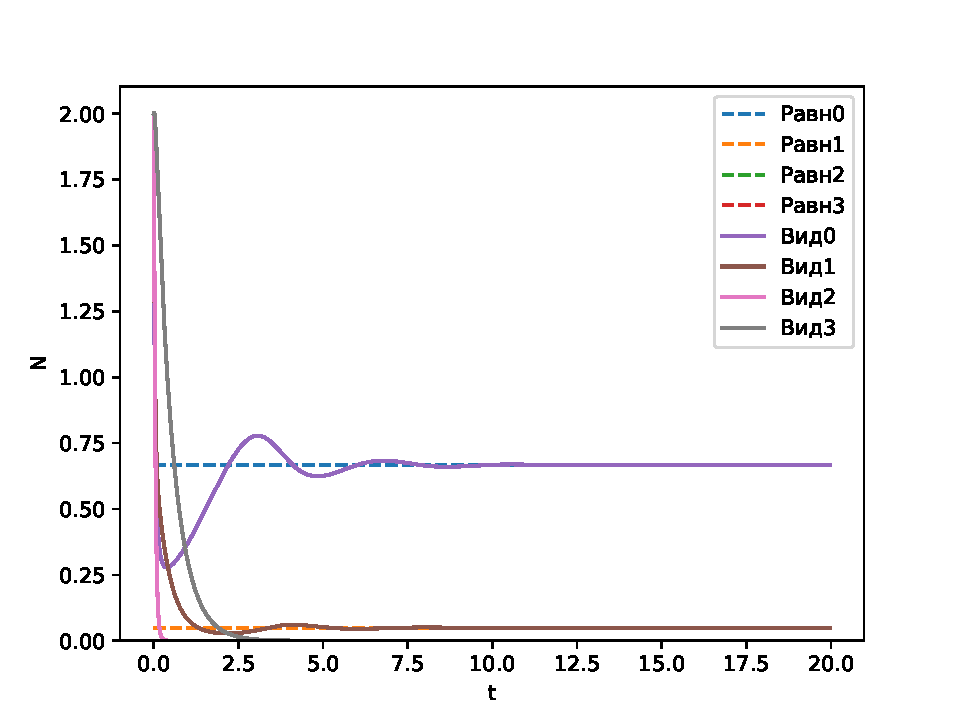
\includegraphics[width=\textwidth]{pictures/cycle/exp1_Q0.5.pdf}
        \caption{\(Q = 0.5\)}
    \end{subfigure}
    \begin{subfigure}[t]{.45\linewidth}
            \centering
            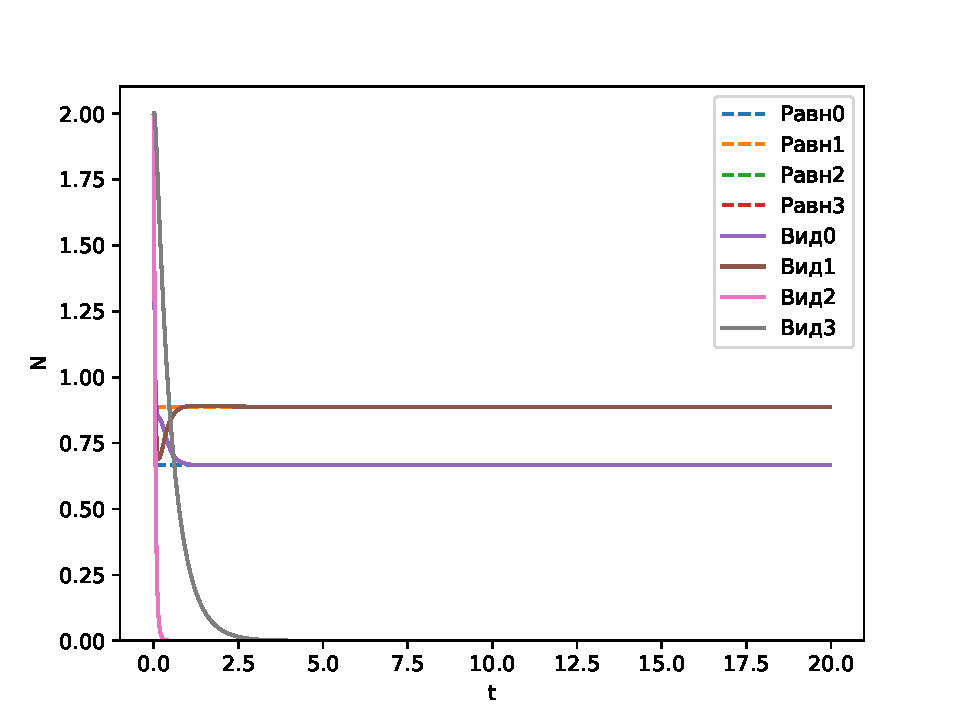
\includegraphics[width=\textwidth]{pictures/cycle/exp1_Q9.pdf}
            \caption{\(Q = 9\)}
        \end{subfigure}
    \caption{Численности видов системы, при \(Q\) близко к концам первого интервала.}  \label{fig:cycle_exp1_q1}
\end{figure}


\begin{figure}[H]
    \centering
    \begin{subfigure}[t]{.45\linewidth}
        \centering
        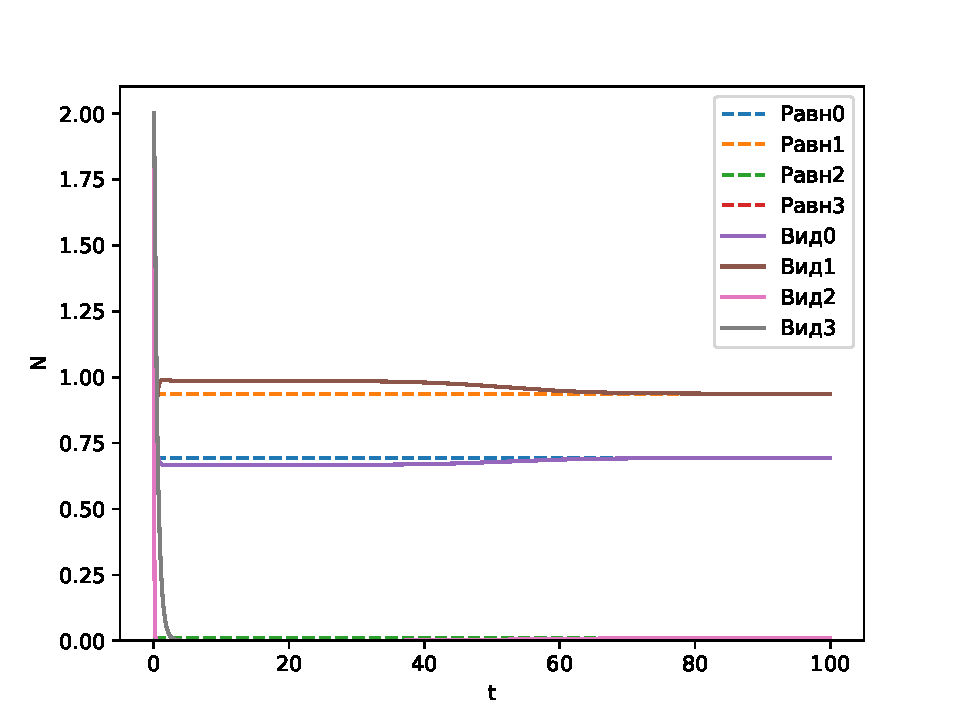
\includegraphics[width=\textwidth]{pictures/cycle/exp1_Q10.pdf}
        \caption{\(Q = 10\)}
    \end{subfigure}
    \begin{subfigure}[t]{.45\linewidth}
            \centering
            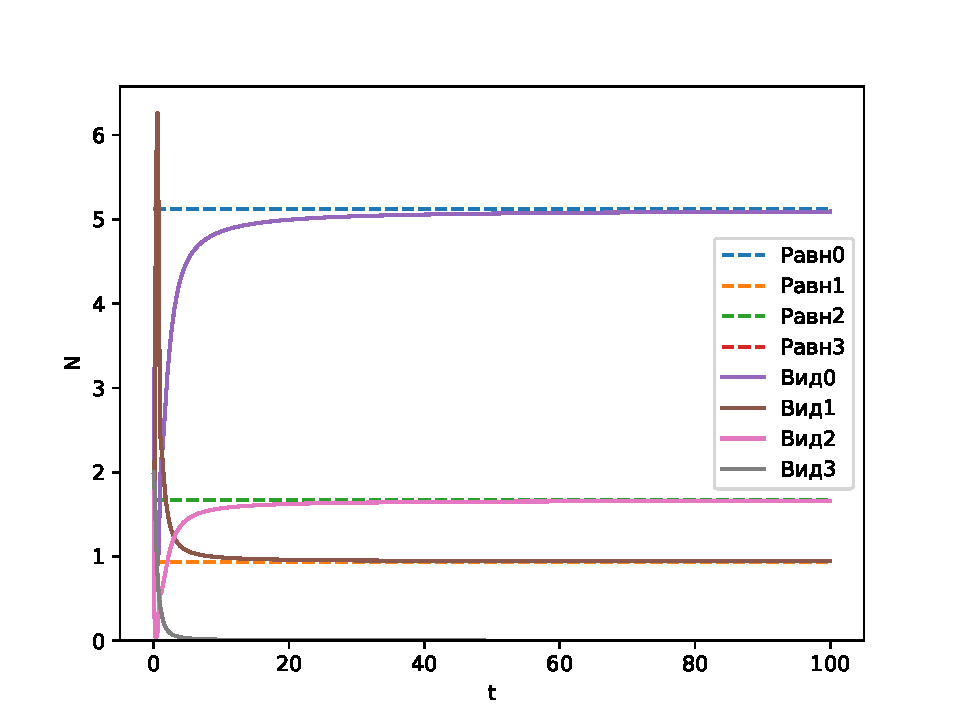
\includegraphics[width=\textwidth]{pictures/cycle/exp1_Q92.pdf}
            \caption{\(Q = 92\)}
        \end{subfigure}
    \caption{Численности видов системы, при \(Q\) близко к концам второго интервала.}  \label{fig:cycle_exp1_q2}
\end{figure}


\begin{figure}[H]
    \centering
    \begin{subfigure}[t]{.45\linewidth}
        \centering
        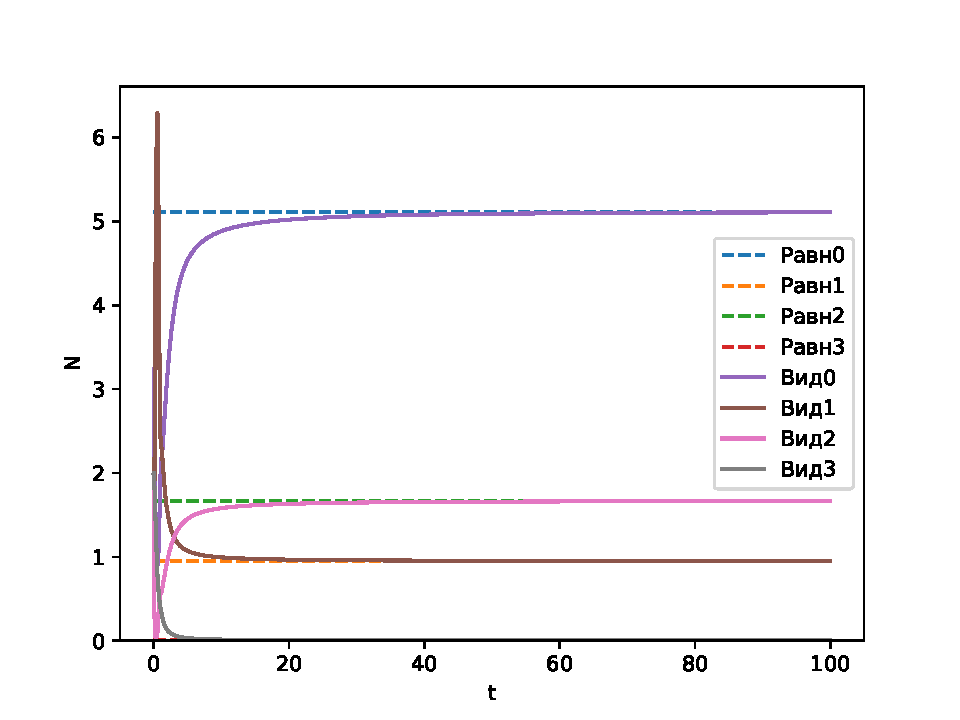
\includegraphics[width=\textwidth]{pictures/cycle/exp1_Q93.pdf}
        \caption{\(Q = 93, \quad N_3 \approx 0.0031\ldots \)}
    \end{subfigure}
    \begin{subfigure}[t]{.45\linewidth}
            \centering
            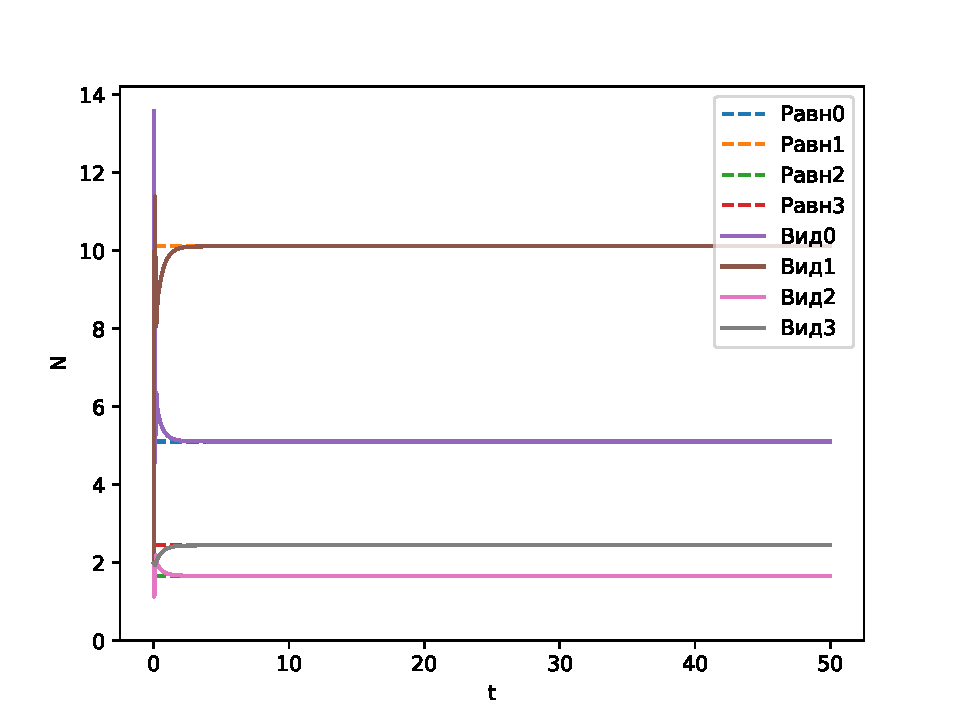
\includegraphics[width=\textwidth]{pictures/cycle/exp1_Q1000.pdf}
            \caption{\(Q = 1000\)}
        \end{subfigure}
    \caption{Численности видов системы, при \(Q\) близко к началу третьего интервала и на некотором отдалении.}  \label{fig:cycle_exp1_q3}
\end{figure}

Для небольшой модели из \(3\)-х видов отличия между проточной и циклической моделью небольшие. Эти обе модели ведут себя похоже и их основное отличие это разные интервалы устойчивости. 

Возьмём эту же модель, но при трофических функциях \( V_i(x) = \alpha_i \arctan x \).

\begin{figure}[H]
    \centering
    \subfigexp{0.5} {pictures/cycle/exp2_Q}{.3}
    \subfigexp{14}  {pictures/cycle/exp2_Q}{.3}
    \subfigexp{15}  {pictures/cycle/exp2_Q}{.3}
    \subfigexp{20}  {pictures/cycle/exp2_Q}{.3}
    \subfigexp{30}  {pictures/cycle/exp2_Q}{.3}
    \subfigexp{30.5}{pictures/cycle/exp2_Q}{.3}
    \subfigexp{40}  {pictures/cycle/exp2_Q}{.3}
    \subfigexp{100} {pictures/cycle/exp2_Q}{.3}
    \subfigexp{1000}{pictures/cycle/exp2_Q}{.3}
\caption{Численности видов системы.}  \label{fig:cycle_exp2}
\end{figure}

В сравнении с экспериментом на рис. \ref{fig:flow_exp2} данная модель при меньших значениях \(Q\) теряет асимптотическую устойчивость и становится периодической. 
    
    \pagebreak

    \section{Незамкнутая ветвящаяся трофическая цепь}
    
    \pagebreak

    \section{Частично замкнутая ветвящаяся трофическая цепь}

    \pagebreak

    \secnonum{Заключение}
    В результате выполнения выпускной квалификационной работы с помощью различных способов исследования устойчивости были получены аналитические выражения, описывающие устойчивость и динамику сообществ вида трофических цепей. В частности, были описаны особенности динамики ветвящейся трофической цепи. Проведённые вычислительные эксперименты подтвердили их согласованность с аналитическими формулами, в том числе и особенность ветвящейся цепи, которая предотвращает рост цепи при определённых условиях.
    
    Полученные результаты могут позволить прогнозировать изменение динамики некоторых структур сообщества при изменении её наблюдаемых параметров, в частности количества доступной питательной энергии.


    \pagebreak

    \renewcommand{\refname}{\centering Список литературы}
\addcontentsline{toc}{section}{Список литературы}
\begin{thebibliography}{1}

    \bibitem{svilog}
        Свирежев, Ю. М. Устойчивость биологических сообществ // Ю. М. Свирежев, Д. О. Логофет -- М.: Наука, 1978.

    \bibitem{barabashin_stability}
        Барбашин Е. А. Введение в теорию устойчивости. -- М.: Наука, 1967, с. 46—47

    % \bibitem{alekseev_karishev}
    %     Кинетические уравнения для описания динамики биоценозов, Алексеев А.А, Карышев И.И.

    % \bibitem{eman}
    %     О некоторых моделях биогеоценозов, Эман Т.И. %% Эман Г.И. ?
    
    \bibitem{quirk_rupert}
        Quirk J. P., Rupert. R Qualitative Economics and the Stability of Equilibrium. -- Rev. Econ. Studies, 1965, 32, №92, p.311-326

    \bibitem{jones_river}
        Jones J. R. E. A further ecological study of a calcareous stream in the «Black Mountain» district of South Wales. — J. Anim. Ecol., 1949, 18, № 2, p. 142—159.


\end{thebibliography}


\end{document}